\documentclass[fleqn,usenatbib,useAMS]{mnras}
\usepackage{mathtools}
\usepackage{natbib}
\bibliographystyle{mnras}
\setcitestyle{authoryear,open={(},close={)}}
\usepackage{graphicx}	% Including figure files
\usepackage{amsmath}	% Advanced maths commands
\usepackage{amssymb}	% Extra maths symbols
\usepackage{multicol}        % Multi-column entries in tables
\usepackage{bm}		% Bold maths symbols, including upright Greek
\usepackage{pdflscape}	% Landscape pages
\usepackage{orcidlink}
\usepackage{url}
\usepackage{cleveref}
\usepackage{booktabs}
\usepackage[flushleft]{threeparttable}
\usepackage{caption}
\usepackage{subcaption}

\newcommand{\kms}{\,km\,s$^{-1}$} % kilometres per second
\newcommand{\bibtex}{\textsc{Bib}\!\TeX} % bibtex. Not quite the correct typesetting, but close enough
%
%
%%%%%%%%%%%%%%%%%%% TITLE PAGE %%%%%%%%%%%%%%%%%%%

% Title of the paper, and the short title which is used in the headers.
% Keep the title short and informative.
\title[]{Can the symmetric \textit{Fermi} and eROSITA bubbles be produced by tilted jets: a proof-of-concept study}

% The list of authors, and the short list which is used in the headers.
% If you need two or more lines of authors, add an extra line using \newauthor
\author[P. H. Tseng et al.]{\large
Po-Hsun Tseng$^{1}$%
\thanks{\href{mailto:zengbs@gmail.com}{zengbs@gmail.com}}%
\orcidlink{https://orcid.org/0000-0002-1868-0660}%
\quad H.-Y. Karen Yang$^{2,3,4,5}$%
\thanks{\href{mailto:hyang@phys.nthu.edu.tw}{hyang@phys.nthu.edu.tw}}%
\orcidlink{https://orcid.org/0000-0003-3269-4660}%
\quad Hsi-Yu Schive$^{1,5,6,7}$%
\thanks{\href{mailto:hyschive@phys.ntu.edu.tw}{hyschive@phys.ntu.edu.tw}}%
\orcidlink{https://orcid.org/0000-0002-1249-279X}%
\quad Chun-Yen Chen$^{8}, $
\quad Tzihong Chiueh$^{1,5,6}$%
\thanks{\href{mailto:chiuehth@phys.ntu.edu.tw}{chiuehth@phys.ntu.edu.tw}}%
\orcidlink{https://orcid.org/0000-0003-2654-8763}%
\\\\
$^{1}$Institute of Astrophysics, National Taiwan University, Taipei 10617, Taiwan\\
$^{2}$Institute of Astronomy, National Tsing Hua University, Hsinchu 30013, Taiwan\\
$^{3}$Department of Physics, National Tsing Hua University, Hsinchu 30013, Taiwan\\
$^{4}$Center for Informatics and Computation in Astronomy, National Tsing Hua University, Hsinchu 30013, Taiwan\\
$^{5}$Physics Division, National Center for Theoretical Sciences, Taipei 10617, Taiwan\\
$^{6}$Department of Physics, National Taiwan University, Taipei 10617, Taiwan\\
$^{7}$Center for Theoretical Physics, National Taiwan University, Taipei 10617, Taiwan\\
$^{8}$Institute of physics, National Taiwan University, Taipei 10617, Taiwan\\
}






% These dates will be filled out by the publisher
\date{\today}

% Enter the current year, for the copyright statements etc.
\pubyear{2022}

% Don't change these lines
\begin{document}
\label{firstpage}
\pagerange{\pageref{firstpage}--\pageref{lastpage}}
\maketitle

% Abstract of the paper
\begin{abstract}
The \textit{Fermi Gamma-Ray Space Telescope} reveals two large bubbles in the Galaxy,\
which extend nearly symmetrically $\sim50^{\circ}$ above and below the Galactic center (GC).\
The recent discovery of giant eROSITA bubbles also shows such a symmetry about the GC, suggesting that they may originate from a single GC activity.\
Previous simulations of bubble formation that invoke active galactic nucleus (AGN) jets\
have assumed that the jets are vertical to the Galactic plane;\
however, in general there does not need to be a correlation between the jet orientation and the rotational axis of the Galactic disk.\
Using three-dimensional (3D) special relativistic hydrodynamic (SRHD) simulations that\
include cosmic rays (CRs) and thermal gas, we show that the interaction between the AGN jets and the thin interstellar medium (ISM) disk is crucial for producing the symmetric \textit{Fermi} and eROSITA bubbles (collectively, Galactic bubbles).\
%We also produce simulated gamma-ray and\
%microwave spectra from the inverse Compton (IC) scattering and synchrotron,\
%and compare them with the observed counterparts in order to verify\
%an oblique AGN jets model.
Specifically, we find that\
(1) the simulated Galactic bubbles are nearly symmetric about the GC albeit\
the bipolar jets are at an angle $45^{\circ}$ with respect to\
the rotational axis of the Galaxy;\
(2) the edge of the eROSITA bubbles corresponds to a forward shock,\
originally driven by oblique bipolar jets emanating from the GC 12.39 million years ago; %,\
%and significantly stretched by the stratified atmosphere afterwards.\
(3) followed by the forward shock is a tangling contact discontinuity,\
which we interpret as the edge of the \textit{Fermi} bubbles\
composed of turbulent and high-temperature ($\sim2$ keV)\
plasma in pressure balance with the external medium;
(4) assuming a leptonic model with spatially uniform CR electron spectrum, we find that the observed gamma-ray and microwave spectra can be reproduced with a best-fit CR power-law index of 2.4.\
The broad agreement between simulated and observed multi-wavelength features suggests that forming the Galactic bubbles by oblique AGN jets is a plausible scenario.
%has thus released a caveat:\
%the jets shall be vertical to the disk normal.
\end{abstract}

% Select between one and six entries from the list of approved keywords.
% Don't make up new ones.
\begin{keywords}
editorials, notices -- miscellaneous
\end{keywords}

%%%%%%%%%%%%%%%%%%%%%%%%%%%%%%%%%%%%%%%%%%%%%%%%%%

%%%%%%%%%%%%%%%%% BODY OF PAPER %%%%%%%%%%%%%%%%%%

% The MNRAS class isn't designed to include a table of contents, but for this document one is useful.
% I therefore have to do some kludging to make it work without masses of blank space.
\begingroup
\let\clearpage\relax
%\tableofcontents
\endgroup
\newpage



\section{Introduction}
The detection of the \textit{Fermi} bubbles \citep{Su2012,Ackermann2014,Narayanan2017},\
two large bubbles symmetrically extending about 50 degrees above and below the Galactic plane,\
is one of the great discoveries of the \textit{Fermi} Large Area Telescope \citep{Atwood2009}.\
The gamma-ray emission of the \textit{Fermi} bubbles is observed in the energy range\
of $\sim$1--100 GeV and has an almost spatially uniform hard\
spectrum, sharp edges and an approximately flat brightness distribution (see \citealt{Yang2018} for a review). Recently, the newly launched eROSITA \citep{Predehl2021} conducted an all-sky X-ray survey with high-spatial resolution and revealed two gigantic bubbles (eROSITA bubbles hereafter) extending to $\sim 80$ degrees in Galactic latitudes, corresponding to an intrinsic size of 14 kpc across \citep{Predehl2020}.\
The remarkable resemblance between the eROSITA and \textit{Fermi} bubbles suggest that they likely share the same origin \citep{Yang2022}.
Their symmetry about the GC further suggests that these Galactic bubbles may be generated by powerful energy injections from the GC, possibly related to nuclear star formation\
\citep{PhysRevLett.106.101102,Carretti2013,Crocker2015,Sarkar2015}
or past AGN activity \citep{Guo2012,Guo2012b,Yang2012,Yang2013,Mou2014,Yang2017}. The latter scenario is what we will focus on in this work.

Previous attempts \citep{Guo2012,Yang2012,Zhang2020}\
to model the formation of the symmetric Galactic bubbles by AGN jets have typically\
assumed that the jets are vertical to the Galactic plane. While there are some observational indications of pc-scale jets from Sgr A* that are found to be perpendicular to the Galactic plane \citep{Li, Zhu}, generally speaking, the AGN jet orientation is determined by the black hole spin and the accretion disk in the black-hole vicinity and does not need to align with the rotational axis of the host galaxy. Indeed, observationally there is a lack of evidence for the alignment between AGN jets and the disk normal \citep[e.g.,][]{Gallimore2006}. The jets are often oblique to the disk normal\
(e.g. NGC 3079, \citealt{Cecil2001}; NGC 1052, \citealt{Dopita2015}),\
and there are even cases in which the jets lie in the plane of the disk (e.g. IC 5063, \citealt{Morganti2015}).\

To this end, the aim of this work is to remove the assumption on jet orientations in the AGN jet models by introducing a dense, thin ISM disk\
that can interact with the central oblique jet,\
in an attempt to resolve the symmetry problem of the Galactic bubbles. More specifically, we use 3D\
SRHD simulations\
involving CR jet injections from the central supermassive black hole (SMBH) in the Galaxy to investigate\
whether the \textit{oblique} jet scenario is able to produce\
the \textit{symmetric} Galactic bubbles. We will verify whether the oblique jet model is\
consistent with the observed features of the Galactic bubbles, including the shape, \
surface brightness, and spectra of the \textit{Fermi} bubbles \citep{Ackermann2014}\
and microwave haze \citep{Dobler_2008,PlanckCollaborationIX2013}.

This paper is organized as follows.\
In Section \ref{Methodology}, we describe the numerical techniques and initial conditions employed.\
In Section \ref{Results}, we first present characteristics of our simulated Galactic bubbles,\
and then discuss how the disk affects the formation of the bubbles.\
We compare the morphology and profiles of the simulated eROSITA bubbles with\
the observed X-ray map in Section \ref{X-ray},\
and present the simulated and observed multi-wavelength spectra of\
the \textit{Fermi} bubbles and microwave haze in Section \ref{sec:gamma-ray-microwave}.\
Finally, the summary and implications of our findings are given in Section \ref{Conclusions}.

\section{Methodology}
\label{Methodology}
  We use the GPU-accelerated SRHD adaptive-mesh-refinement (AMR) code \textsc{gamer-sr} developed at the\
  National Taiwan University\
  (\citeauthor{gamer-1} \citeyear{gamer-1}, \citeyear{gamer-2}; \citeauthor{tseng2021} \citeyear{tseng2021})\
  to carry out the simulations of the Galactic bubbles formed by CR and relativistic-fluid injections from the GC.

  The governing equations solving the special relativistic ideal fluid\
  including CR advection, and dynamical coupling between the thermal gas and CRs without CR diffusion\
  can be written in a succinct form as


  \begin{subequations}
    \label{governing-eq}
    \begin{align}
     &\partial_{t} D+\partial_{j} \left(DU^{j}/\gamma\right)=0,\label{D evolution}\\
     &\partial_{t} M^{i}+\partial_{j} \left(M^{i}U^{j}/\gamma+p_{\text{total}}\delta^{ij}\right)=\
     -\rho\partial_{i}\Phi,\label{M evolution}\\
     &\partial_{t} \tilde{E}+\partial_j \left[\left(\tilde{E}+p_{\text{gas}}\right)U^{j}/\gamma\right]=0, \label{E evoltion}\\
     &\partial_{t} \left(\gamma e_{\text{cr}}\right) + \partial_{j} \left(e_{\text{cr}}U^{j}\right)=\
     -p_{\text{cr}} \partial_{j} U^{j},\label{E evolution}
    \end{align}
  \end{subequations}


  where the five conserved quantities of gas $D$, $M^{i}$, and $\tilde{E}$ are the mass density,\
  the momentum densities, and the reduced energy density, respectively.\
  The reduced energy density is defined by subtracting the rest mass energy density of gas\
  from the total energy density of gas.\
  $\gamma$ and $U^{j}$ are the temporal and spatial component of four-velocity of gas.\
  $\rho$ is the gas density in the local rest frame defined by $D/\gamma$.\
  $p_{\text{gas}}$ is the gas pressure.\
  $p_{\text{cr}}$ and $e_{\text{cr}}$ are the CR pressure and CR energy density measured in the local rest frame.\
  $p_{\text{total}}$ is the sum of $p_{\text{gas}}$ and $p_{\text{cr}}$.\
  Note that we simply replace $p_{\text{total}}$ by $p_{\text{gas}}$ in this paper\
  as we have assumed $p_{\text{cr}}\ll p_{\text{gas}}$.\
  $\Phi$ is a gravitational potential.\
  $c$ is the speed of light, and $\delta^{ij}$ is the Kronecker delta notation.\
  Throughout this paper, Latin indices run from 1 to 3, except when stated otherwise. The set of Eq. \ref{governing-eq} is closed by using the Taub-Mathews equation of state \citep[EoS;][]{Taub,TM_EOS}\
  that approximates the exact EoS \citep{Synge} for ultra-relativistically\
  hot gases coexisting with non-relativistically cold gases.
  %Since the relativistic fluid ejected by the jet source\
  %is quickly stalled off and slowed down by the dense ISM,\
  %and the relativistic fluid\
  %accounts for a little minority of total mass inside the simulation box,\
  %we still use the Newtonian gravity to attack this problem.

  \textsc{gamer-sr} adopts a new algorithm \citep{tseng2021} to convert between\
  primitive ($\rho$, $U^{j}$, $p$) and conserved variables ($D$, $M^{j}$, $\tilde{E}$),\
  significantly reducing numerical errors caused by catastrophic cancellations\
  that commonly occur within the regions with high Mach number flows. e.g., jet-ISM interaction zones.\
  \textsc{gamer-sr} also adaptively and locally reduce the min-mod coefficient\
  \citep{tseng2021} within the failed patch group rarely occurring in the SRHD solver,\
  new patches allocations, and ghost-zone interpolations.\
  In this manner, we provide an elegant approach to avoid the use of pressure/density floor,\
  being unnatural but widely used in almost publicly available codes.\

  In order to track the evolution of CRs injected by the AGN jets and make predictions of the non-thermal radiation they produce, we adopt the CR hydrodynamic formalism and model the CRs as a second fluid \citep{Zweibel2013}. The approach is similar to previous works of \cite{Guo2012} and \cite{Yang2012}, but generalized to CRs that couple with thermal gas moving with relativistic speeds. The detailed implementations in \textsc{gamer-sr} and tests of the algorithm can be found in a forthcoming paper \citep[][in prep.]{Chen2022}. In this approach, the CRs are treated as a single species without distinctions between CR electrons and protons,\
  and the CR energy density $e_{\text{cr}}$ is evolved according to Eq. \ref{E evolution}.
  The CRs are advected with the thermal gas and can have adiabatic compression and expansion with the gas. Also, we do not simulate the spectral evolution of the CRs and assume that the CR-to-gas pressure ratio is much less than 1 so that\
  the contribution of CR pressure gradient to the momentum of the gas can be ignored\
  (we will see that the ratio is around 0.1--0.2 throughout the simulations). Note that, although our later calculations of the non-thermal spectra are based on the leptonic model, only a small fraction of the simulated CRs is required to produce the observed gamma-ray and microwave emission \citep{Yang2013}.
{\color{red} KY: Is this also true in the current simulations? That is, from the simulated CR energy densities, did you have to apply a normalization constant to match with the observed gamma-ray/microwave spectra? PH: We have reached a consensus on this matter on Slack!}
Therefore, in the simulations we have neglected the cooling of CRs because it should have a negligible impact on the overall dynamics.
  %Over and above, we neglect the cooling and heating processes of CRs,\
  %such as energy losses due to synchrotron and inverse Compton emission,\
  %and CR reacceleration in shocks/turbulences.

  As stressed by \citet{Yang2012}, CR diffusion with a canonical diffusion coefficient of $\kappa \sim 3\times 10^{28}$ cm$^2$ s$^{-1}$ in the Galaxy has a minor effect\
  on the overall morphology of the \textit{Fermi} bubbles as it
  only acts to smooth the CR distributions on the scales of $l \sim \sqrt{\kappa t} \sim 0.3\ (t/1 {\rm Myr})$ kpc. Including anisotropic CR diffusion can also help to sharpen the edges of the bubbles due to interplay between the magnetic field\
  and anisotropic CR diffusion with suppressed perpendicular diffusion across the bubble surface. As for the magnetic field, \cite{Yang2013} has found that the magnetic field within the \textit{Fermi} bubbles needs to be amplified to comparable values to the ambient field in order to reproduce the microwave haze emission. We thus directly adopt the exponential model for the magnetic field distribution in our calculation for the haze (see descriptions in Section \ref{sec:model}).
%  Furthermore, the magnetic field within the \textit{Fermi} bubbles should be weak due to\
%  adiabatic expansion, and thus the fields has\
%  a little effect on the overall dynamics.
   For the above reasons, we have ignored CR diffusion and the magnetic field in the simulations.\


  \subsection{The Galactic and Disk Models} \label{sec:model}
  As a proof-of-concept study, we approximate conventionally axisymmetric stellar potential of Milky Way\
  by a plane-parallel potential that is symmetric about the Galactic plane, $z=0$,\
  in a simulation domain of\
  $14\times14\times28$ kpc, slightly larger than the size of eROISTA bubbles. The plane-parallel potential is fixed throughout our simulations and given by
  \begin{equation}
    \Phi_{\text{total}}(z) = \Phi_{\text{bulge}}(z) + \Phi_{\text{halo}}(z),
  \end{equation}
  where
  \begin{equation}
    \Phi_{\text{bulge}}(z)=\
    2\sigma^2_{\text{bulge}}\
    \ln\cosh\left(z\sqrt{\frac{2\pi G\rho_{\text{bulge}}^{\text{peak}}}{\sigma^2_{\text{bulge}}}}\right)
  \end{equation}
  is the potential of an isothermal slab mainly contributed by stars around the Galactic bulge, and\
  $\Phi_{\text{halo}}(z)=v^2_{\text{halo}}\ln\left(z^2+d^2_{\text{h}}\right)$\
  is a plane-parallel logarithmic dark halo potential.

  With the isothermal assumption and the condition of hydrostatic equilibrium within the total potential of the disk and halo, as well as pressure equilibrium between the isothermal disk and the halo gas, we can write down the steady-state gaseous density distribution as\
  \begin{subequations}
  \begin{align}
     \displaystyle \rho_{\text{isoDisk}}(z) = \rho_{\text{isoDisk}}^{\text{peak}}
     \exp\left[-\frac{\Phi_{\text{total}}(z)}{k_{B}T_{\text{isoDisk}}/m_{\text{p}}}\right]&\label{isothermal-disc-density}\\
     \text{, if $|z| < z_{0}$,}& \nonumber \\
     \nonumber\\
     \displaystyle \rho_{\text{atmp}}(z) = \rho_{\text{atmp}}^{\text{peak}}
     \exp\left[-\frac{\Phi_{\text{total}}(z)}{k_{B}T_{\text{atmp}}/m_{\text{p}}}\right]&\label{isothermal-atmp-density}\\
     \text{, otherwise,}& \nonumber
  \end{align}
  \label{disc-atm-sys}
  \end{subequations}
  where $m_{\text{p}}$ is the proton mass,\
  $T_{\text{isoDisk}}$ and $T_{\text{atmp}}$ are the temperature of the isothermal disk and the ambient atmosphere, and\
  $\rho_{\text{isoDisk}}^{\text{peak}}$ and $\rho_{\text{atmp}}^{\text{peak}}$ are the peak density\
  of the disk and the atmosphere at $z=0$, respectively.

  We tabulate parameters adopted for the Galactic model in \Cref{table-parameters},\
  except for $\rho_{\text{atmp}}^{\text{peak}}$ that\
  can be derived from the other known parameters and the pressure equilibrium condition\
  at the interfaces $(z=\pm z_{0})$ between the disk and the atmosphere. The density profile of Eq. \ref{disc-atm-sys} is shown in Fig. \ref{fig__initial-density-profile}.\
  Beyond the core radius ($\sim 2 \text{ kpc}$) the gas density decreases rapidly as a power-law.


  \begin{figure}
    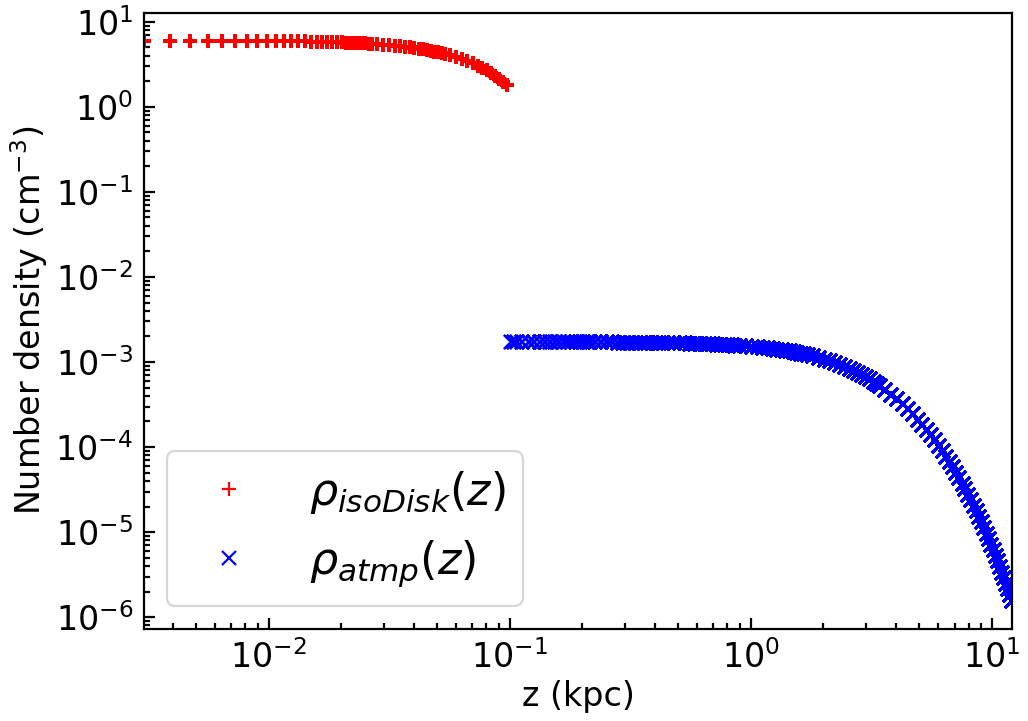
\includegraphics[width=\columnwidth]{figures/fig__initial-density-profile.png}
    \caption{The density profile of the isothermal disk (red pluses) and\
             the ambient atmosphere (blue crosses) along the positive $z$-axis.\
             The density distribution is derived from the condition of hydrostatic equilibrium.\
             The gas at the interface between the isothermal disk\
             and the atmosphere at $z=0.1$ is in pressure equilibrium.}
    \label{fig__initial-density-profile}
  \end{figure}



  To compute the predicted synchrotron radiation as a function of position,\
  we adopt the default exponential magnetic field in \textsc{galprop} \citep{Strong2007}
  that obeys the following spatial dependence:\

  \begin{equation}
     |\mathbf{B}(R, z)|=B_{0}\exp\left[-\frac{z}{z_{0}}\right]\exp\left[-\frac{R}{R_{0}}\right],
     \label{magnetic-field}
  \end{equation}


  where $R=\sqrt{x^{2}+y^{2}}$, $B_{0}$ is the average field strength at the GC,\
  and $z_{0}$ and $R_{0}$ are the characteristic scales in the vertical and radial\
  directions, respectively. We adopt $z_{0} = 2$ kpc and $R_{0} = 10$ kpc, which\
  are best-fitting values in the \textsc{galprop} model to reproduce the\
  observed large-scale 408 MHz synchrotron radiation in the Galaxy.\
  We choose $B_{0} = 50$ $\mu$G based on the observed field strength at the\
  GC \citep{Crocker2010}.

  % The dispersion:
  %   2010-Comparing the statistics of interstellar turbulence in simulations and observations
  %   2011-RELATIVISTIC JET FEEDBACK IN EVOLVING GALAXIES


  \subsection{The Clumpy Multiphase Interstellar Medium}

  A crucial component in our work is the clumpy ISM disk initialized by\
  the publicly available pyFC code
  \footnote{\url{https://pypi.python.org/pypi/pyFC}}.
  pyFC randomly generates dimensionless 3D scalar field $f(\bold{x})$\ % that is clumpy and porous.
  that obeys the log-normal probability distribution\
  with mean $\mu$ and dispersion $\sigma$,\
  and follows the power-law Kolmogorov spectrum
  \begin{equation}
    D(\bold{k})=\int k^{2} \hat{f}(\bold{k})\hat{f}^{*}(\bold{k})d\Omega \propto k^{-\beta},
    \label{Kolmogorov-spectrum}
  \end{equation}
  where $\hat{f}(\bold{k})$ is the Fourier transform of $f(\bold{x})$.\
  The spectrum $D(\bold{k})$ in the Fourier space is characterized by a power-law index $\beta=5/3$,\
  a Nyquist limit $k_{\text{max}}$, and a lower cutoff wave number $k_{\text{min}}$.
  $k_{\text{max}}$ is one-half of the spatial resolution within the disk,\
  and $k_{\text{min}}$ is 375.0, corresponding to the maximum size of an individual clump of $\sim 20$ pc.\
  \citet{LA2002} and \citet{Wagner2012} have outlined a detailed procedure\
  for constructing a clumpy scalar field, and we refer the readers for more information.

  The density of the clumpy disk can then be obtained by taking the scalar products of\
  $f(\bold{x})$ with $\rho_{\text{isoDisk}}(z)$ over all cells within the disk, i.e.,\
  $\displaystyle\rho_{\text{ismDisk}}(\bold{x}) =\
  f(\bold{x}) \rho_{\text{isoDisk}}(z)$.\
  Also, the thermal pressure equilibrium within the clumpy disk implies that the temperature of the disk is
  $\displaystyle T_{\text{ismDisk}}(\bold{x}) =\
  T_{\text{isoDisk}}(z)\rho_{\text{isoDisk}}(z)/\rho_{\text{ismDisk}}(\bold{x})$. The last category in \Cref{table-parameters} summarizes the parameters of the clumpy disk and their references.

  On the basis of this setup, we cover the AMR base level with\
  $16\times16\times32$ root cells, refined progressively on the mid-plane at $z=0$\
  based on the gradient of density.\
  We also restrict the refinement level at 7 within the disk so that\
  a molecular cloud can be adequately resolved by approximately 30 cells along their diameter of 20 pc. We plot the volume filling factor as a function of\
  initial number density within the disk without the jet source in Fig. \ref{fig__numberDensityHistogram},\
  and show a close-up view of the\
  pressure, temperature, and number density slices
  in the $y-z$ plane through the center of the disk in Fig. \ref{fig__zoom-in-disc}.

  \begin{figure}
      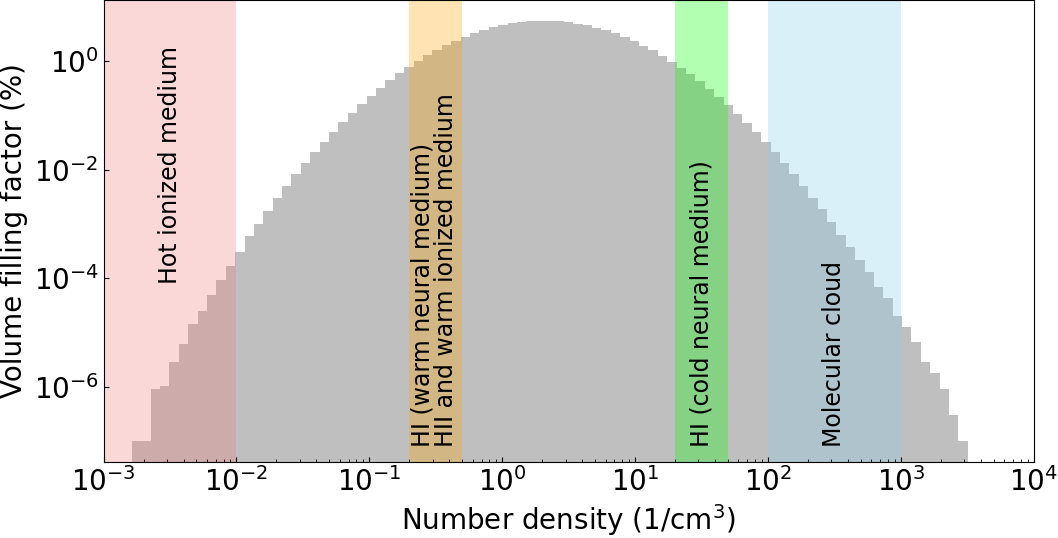
\includegraphics[width=\columnwidth]{figures/fig__numberDensityHistogram.png}
    \caption{The volume filling factor as a function of\
             initial number density within the disk without the jet source.\
             The vertical bands from left to right depict the allowable number densities \citep{peak-ism-density} for\
             hot ionized, warm neutral (WNM), warm ionized (WIM), cold neutral mediums (CNM), and molecular clouds.}
      \label{fig__numberDensityHistogram}
  \end{figure}

  \begin{figure}
    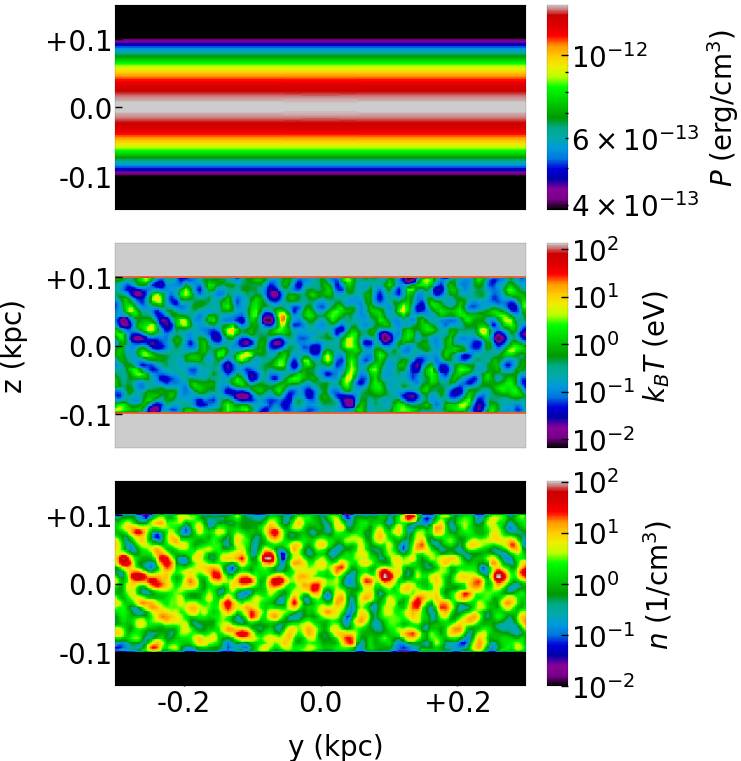
\includegraphics[width=\columnwidth]{figures/fig__zoom-in-disc.png}
    \caption{Close-up view of the initial\
             pressure (top), temperature (middle), and number density (bottom) slices\
             in the $y-z$ plane through the center of the disk.
             }
    \label{fig__zoom-in-disc}
  \end{figure}

\begin{table*}
\raggedright
\caption{Parameters of the disk, atmosphere, and gravitational potential in the simulations.}
\label{table-parameters}
\begin{tabular}{@{}llrc@{}}
\toprule[1pt]\midrule[0.3pt]
Parameter                             & Description                    & Value                                &  Reference                     \\ \midrule
{\bf Static stellar potential }       &                                &                                      &                                \\
$\sigma_{\text{bulge}}$               & Velocity dispersion of bulge   & 100 km s$^{-1}$                & \citep{velocity-dispersion-MW} \\
$\rho_{\text{bulge}}^{\text{peak}}$   & Peak average density of bulge  & $4\times 10^{-24}$ g cm$^{-3}$ &   N/A                          \\ \hline
{\bf Static dark halo potential }     &                                &                                      &                                \\
$v_{\text{halo}}$                     & Characteristic velocity        & 131.5 km s$^{-1}$              & \citep{Johnston1995}           \\
$d_{\text{h}}$                        & Core radius                    & 12 kpc                               & \multicolumn{1}{c}{''}         \\ \hline
{\bf Atmosphere }                     &                                &                                      &                                \\
$T_{\text{\text{atmp}}}$              & Temperature of atmosphere      & $10^{6}$ K                           & \citep{temperature-MW}         \\ \hline
{\bf Isothermal disk }                &                                &                                      &                                \\
$z_{0}$                               & Scale height of disk           & 100 pc                               & \citep{peak-ism-density}       \\
$T_{\text{\text{isoDisk}}}$           & Temperature of disk            & $10^{3}$ K                           & \multicolumn{1}{c}{''}         \\
$\rho_{\text{isoDisk}}^{\text{peak}}$ & Peak density of disk      & $10^{-23}$ g cm$^{-3}$         & \multicolumn{1}{c}{''}         \\ \hline
{\bf Clumpy disk }                    &                                &                                      &                                \\
$k_{\text{min}}^\dagger$            & Cutoff wave number             & 375.0                                & \citep{peak-ism-density}       \\
$\mu$                                 & Mean of scalar field           & 1.0                                  &   N/A                          \\
$\sigma^\ddag$                 & Dispersion of scalar field     & 5.0                                  & \citep{Federrath2010}          \\
$\beta$                               & Power law index                & -5/3                                 &   N/A                          \\ \midrule
\end{tabular}
\begin{tablenotes}
      \raggedright
      \item  $\dagger$  $k_{\text{min}}=375.0$ leads to the size of an individual molecular cloud of $\sim 100$ pc.
      \item  $\ddag$ In numerical simulations of turbulence,\
             \citet{Federrath2010} find $\sigma\sim 3.6$ and 35 for solenoidal (divergence-free)\
             and compressive (curl-free) driving force,\
             respectively, so that our adopted value of 5 is closer to their solenoidal result.
    \end{tablenotes}
\end{table*}

%

\subsection{Oblique jets}

  We simulate the jets emanating from the GC with an inclination angle\
  $45^{\circ}$ with respect to the Galactic plane\
  in order to alleviate the constraint that\
  the jet direction must be perpendicular to the Galactic plane, and in particular to\
  investigate how the dense disk affects the bubble formation.


  We use the following quantities to characterize the jets:
  the density contrast between the thermal gas contained in the jet source and the ambient gas,\
  $\rho_{\text{jet}}/\rho_{\text{amb}}=10^{-3}$,\
  the temperature contrast, $T_{\text{jet}}/T_{\text{amb}}=2\times10^{4}$,\
  the CR-to-gas pressure ratio of 0.18,\
  and the flow 4-velocity inside the jet source along the jet axis, $\beta\gamma = 0.6$.\
  The jet power is thus $3.2\times 10^{42}$ erg s$^{-1}$, resulting in an Eddington ratio of 0.008.\
  Note that since we inject the jets at the center of the clumpy disk,\
  we define the atmosphere gas density by the peak density of\
  the isothermal disk on the mid-plane $z=0$ (i.e. $\rho^{\text{peak}}_{\text{isoDisk}}$),\
  as opposed to the \textit{clumpy} density around the jet source.


  The bipolar jets are constantly ejected from a cylindrical source starting from the beginning of simulation ($t=0$)\
  and suddenly quenched at $t=1.2$ Myr before fully breaking out the disk.\
  Without quenching, the Galactic bubbles at the present time would be asymmetric about the Galactic plane.
  The jet duration allows the total ejected energy to be $1.2\times10^{56}$ erg, \
  within the range of estimates obtained by \citet{Predehl2020} between\
  $8\times10^{55}$ erg and $1.3\times10^{56}$ erg.



  The diameter and height of cylindrical source are 4 pc,\
  leading to a source volume ($\sim 50 \text{ pc}^{3}$)\
  much smaller than that of an individual clump by a factor of $\sim 83$.\
  By intentionally reducing the volume ratio of the jet source to an individual clump,\
  we can mitigate the effect of the randomness of the clumps on the bubbles.\
  Moreover, we resolve the jet source with the highest refinement level of 11,\
  bringing the finest spatial resolution up to 0.4 pc.\

\section{Results}
\label{Results}

\subsection{Morphology and properties of Galactic bubbles}

 Fig. \ref{fig__jetI5+ismSeed3-45deg} shows\
 the slices of pressure (top), temperature (middle), number density (bottom)\
 at the end of simulation $t=12.39$ Myr.\
 The slices pass through the bipolar jet source injecting along $z=-y$ direction.

 The fiducial run (Fig. \ref{fig__jetI5+ismSeed3-45deg-a})\
 with the initial condition specified in Section \ref{Methodology}\
 shows that the edge of the outermost bubbles is a forward shock,\
 expanding to 12.5 kpc above and below the Galactic plane,\
 with a semiminor axis about 6.8 kpc on the plane.\
 The overall extent of the outermost bubbles is comparable to\
 the two spherical objects of a radius of 6-7 kpc estimated by \citet{Predehl2020}\
 for modeling the eROSITA bubbles.\
 The temperature profile (left middle panel in Fig. \ref{fig__profile}) along the positive $z$-axis in\
 Fig. \ref{fig__jetI5+ismSeed3-45deg} indicates that\
 the temperature of the smooth region (purple band in Fig. \ref{fig__profile})\ %emitting X-ray\
 is around 0.3-0.5 keV, similar to 0.3 keV observed by \citet{Miller2016} and \citet{Kataoka2018}. {\color{red} (KY: What did these observations constrain exactly?
PH: It is 0.3 keV. I have added this number in the context. See: ``...follows from the Rankine-Hugoniot condition for the temperature increase from about 0.2 keV outside the bubbles to around 0.3 keV inside$^{7,19}$" in \citealt{Predehl2020})}

 Followed by the forward shock is a turbulent and hot plasma extending to a height of $\sim 8$ kpc (Fig. \ref{fig__profile}).\
 The extent of the turbulent plasma approximately agrees with\
 that of the observed \textit{Fermi} bubbles \citep{Su2010}.
 Also, the temperature of the plasma is around 2 keV,\
 comparable to few keV inside the \textit{Fermi} bubbles\
 estimated by observing X-ray absorption lines through the hot\
 gaseous halo along many different sight lines in the sky \citep{Miller_2013}.\
 We also note that the turbulent, hot plasma is in pressure balance with the external medium,\
 suggesting the outer edge of the \textit{Fermi} bubbles\
 is a contact discontinuity rather than a shock \citep{Zhang2020}.


 An interesting feature found in our simulations is that there are a pair of innermost bubbles\
 (dashed box in the top panel of Fig. \ref{fig__jetI5+ismSeed3-45deg-a})\
 extending out from the GC on either side of the thin disk.\
 The innermost bubbles are cold (1-10 eV), dense ($10^{-4}$--$10^{-2}$ cm$^{-3}$),\
 and underpressured with respect to the turbulent plasma.\
 The close-up view (right column in Fig. \ref{fig__profile}) of the vertical profiles\
 and slices (Fig. \ref{fig__innerbubbles})\
 demonstrate that there is a sharp pressure jump at the edge of the innermost bubbles at $z=3.62$ kpc,\
 indicating that the innermost bubbles are an expanding reverse shock.\ {\color{red} KY: Is it verified that the reverse shock is expanding outward? PH: Yes. I have checked that with multiple slices in different time. The reverse shock is expanding outward.}
 The high-density upstream of the reverse shock requires\
 an even higher density downstream.\
 Continuing outward, there exists a dense shell before the gas density drops to values further downstream.
 %Continuing outward, the higher density must match with low density further downstream;\
 %thus there exists a dense shell.\
 The turbulent plasma is therefore bracketed between the downstream of reverse shock\
 and of the outermost forward shock, thus heating the turbulent plasma up considerably.

 We stress that either the outermost shock, turbulent plasma, or innermost bubbles\
 are symmetric about the Galactic plane despite that the jets are tilted to the disk normal\
 at an angle of $45^{\circ}$.

 In addition to the fiducial run, in Fig. \ref{fig__jetI5+ismSeed3-45deg} we also show the slices of various gas properties at $t=12.39$ Myr in different Galactic environments. We compare the clumpy disk (Fig. \ref{fig__jetI5+ismSeed3-45deg-a})\
 with the smooth disk in a stratified atmosphere (Fig. \ref{fig__jetI5+ismSeed3-45deg-b}; the initial density profile is shown in Fig. \ref{fig__initial-density-profile}). \
 The results show that the clumpiness of\
 the dense disk has an insignificant effect\
 on the overall dynamics of bubbles. However, the outermost bubbles arising from the smooth disk\
 in a uniform atmosphere (Fig. \ref{fig__jetI5+ismSeed3-45deg-c}) is quasi-spherical,\
 suggesting that the stratification facilitates the elongation of the outermost bubbles significantly. Fig. \ref{fig__jetI5+ismSeed3-45deg-c} and \ref{fig__jetI5+ismSeed3-45deg-d}\
 reveal that the development of the innermost bubbles\
 is always associated with the disk. Also, without the disk (Fig. \ref{fig__jetI5+ismSeed3-45deg-d}),\
 the outermost bubbles and the turbulent plasma would be oblique,\
 indicating that the dense disk is crucial for the production of symmetric Galactic bubbles.\


 \begin{figure}%
      \captionsetup[subfigure]{labelformat=simple}
      \begin{subfigure}[b]{0.2\linewidth}%
         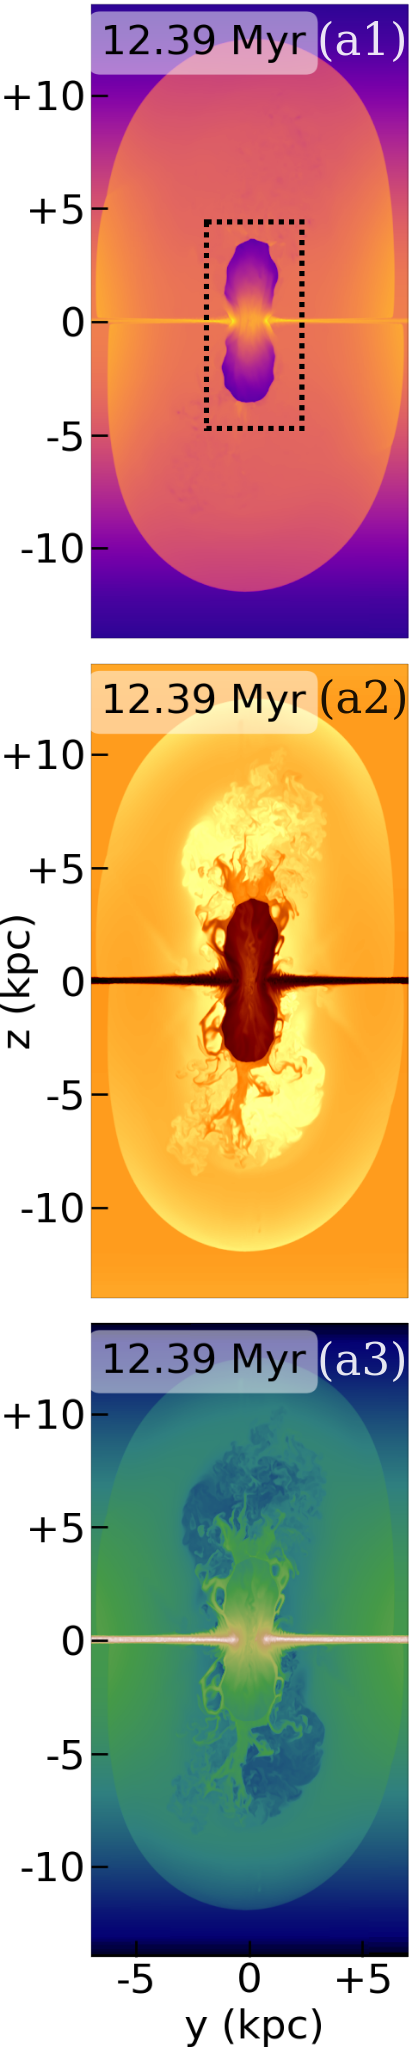
\includegraphics[height=10cm]{figures/fig__jetI5+ismSeed3-45deg-a}%
         \caption{}%
         \label{fig__jetI5+ismSeed3-45deg-a}%
      \end{subfigure}%
      \hspace{10pt}%
      \begin{subfigure}[b]{0.2\linewidth}%
         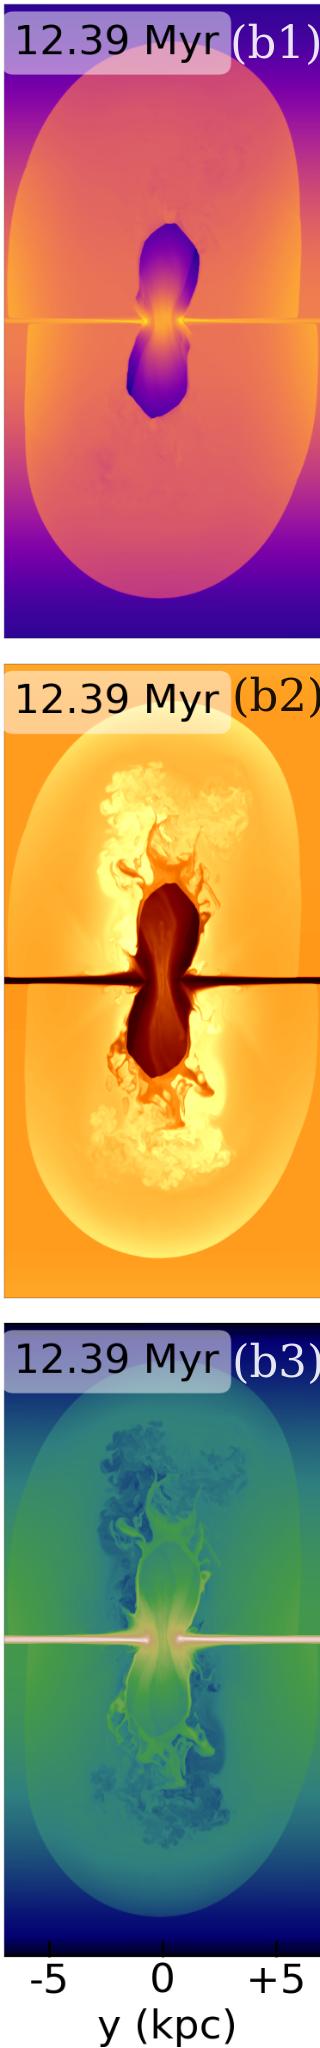
\includegraphics[height=10cm]{figures/fig__jetI5+ismSeed3-45deg-b}%
         \caption{}%
         \label{fig__jetI5+ismSeed3-45deg-b}%
      \end{subfigure}%
      \hspace{-2pt}%
      \begin{subfigure}[b]{0.2\linewidth}%
         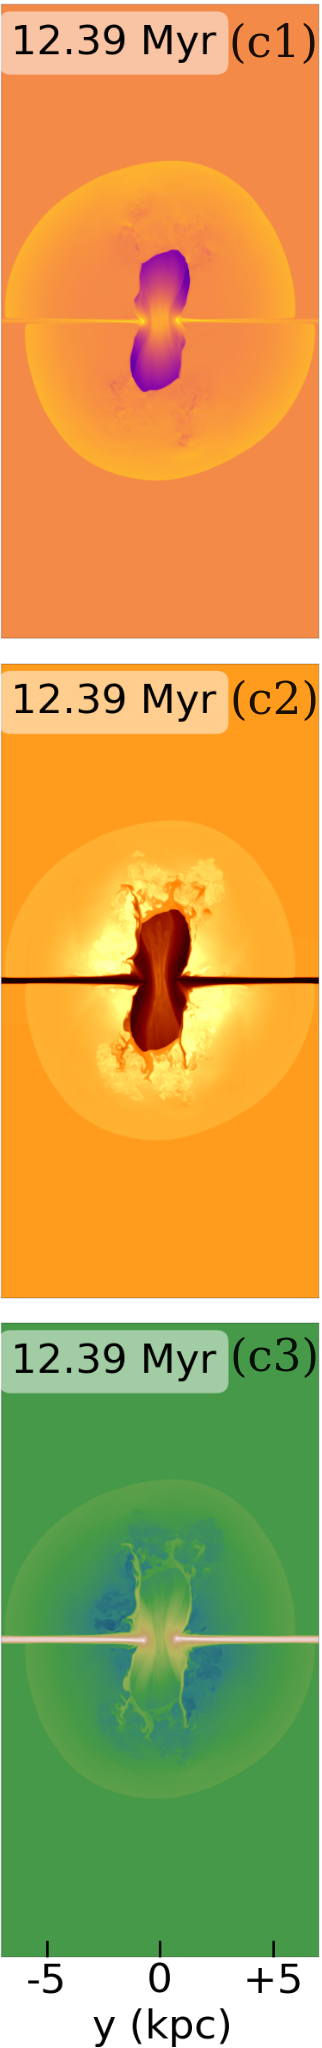
\includegraphics[height=10cm]{figures/fig__jetI5+ismSeed3-45deg-c}%
         \caption{}%
         \label{fig__jetI5+ismSeed3-45deg-c}%
      \end{subfigure}%
      \hspace{-2pt}%
      \begin{subfigure}[b]{0.2\linewidth}%
         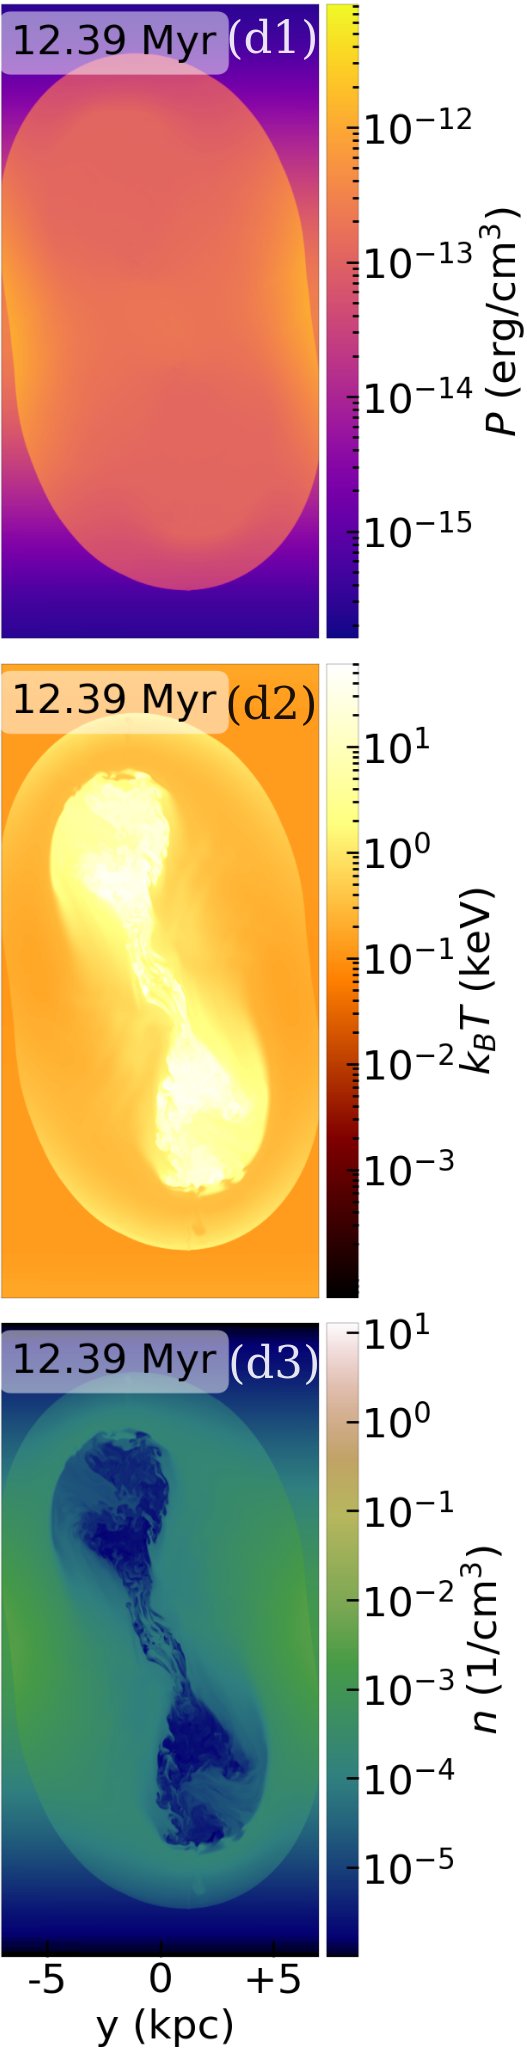
\includegraphics[height=10cm]{figures/fig__jetI5+ismSeed3-45deg-d}%
         \caption{}%
         \label{fig__jetI5+ismSeed3-45deg-d}%
     \end{subfigure}%
      \caption{
             The slices of pressure (top), temperature (middle), and number density (bottom)\
             at the end of simulation $t=12.39$ Myr.\
             The slices pass through a bipolar jet source injecting along $z=-y$ direction\
             for a duration $t=0$--$1.2$ Myr.\
             Comparison between the clumpy (Fig. \ref{fig__jetI5+ismSeed3-45deg-a})\
             and the smooth disks (Fig. \ref{fig__jetI5+ismSeed3-45deg-b}) in a stratified atmosphere\
             shows that the initial density distribution of the dense disk has an insignificant effect\
             on the overall dynamics of bubbles. However, the outermost bubbles arising from the smooth disk\
             in an uniform atmosphere (Fig. \ref{fig__jetI5+ismSeed3-45deg-c}) is nearly spherical,\
             suggesting that the stratification facilitates the elongation of the outermost bubbles significantly.\
             Fig. \ref{fig__jetI5+ismSeed3-45deg-c} and \ref{fig__jetI5+ismSeed3-45deg-d}\
             reveal that the development of the innermost bubbles\
             is always associated with the disk. Also, without the disk (Fig. \ref{fig__jetI5+ismSeed3-45deg-d}),\
             the outermost bubbles and the turbulent plasma would be oblique,
             indicating that the dense disk is crucial for the production of symmetric Galactic bubbles.\ {\color{red} KY: Consider reducing the caption as it is essentially the same as the text. PH: Thanks! I would say figures and captions must be self-explanatory i.e. always summarize the key conclusions of this figure instead of just describing how this figure is plotted. This is the reason why the caption is a little long... \textasciicircum\textasciicircum"}
      }
      \label{fig__jetI5+ismSeed3-45deg}
 \end{figure}%


 \begin{figure}%
      \begin{subfigure}[t]{0.5\linewidth}%
         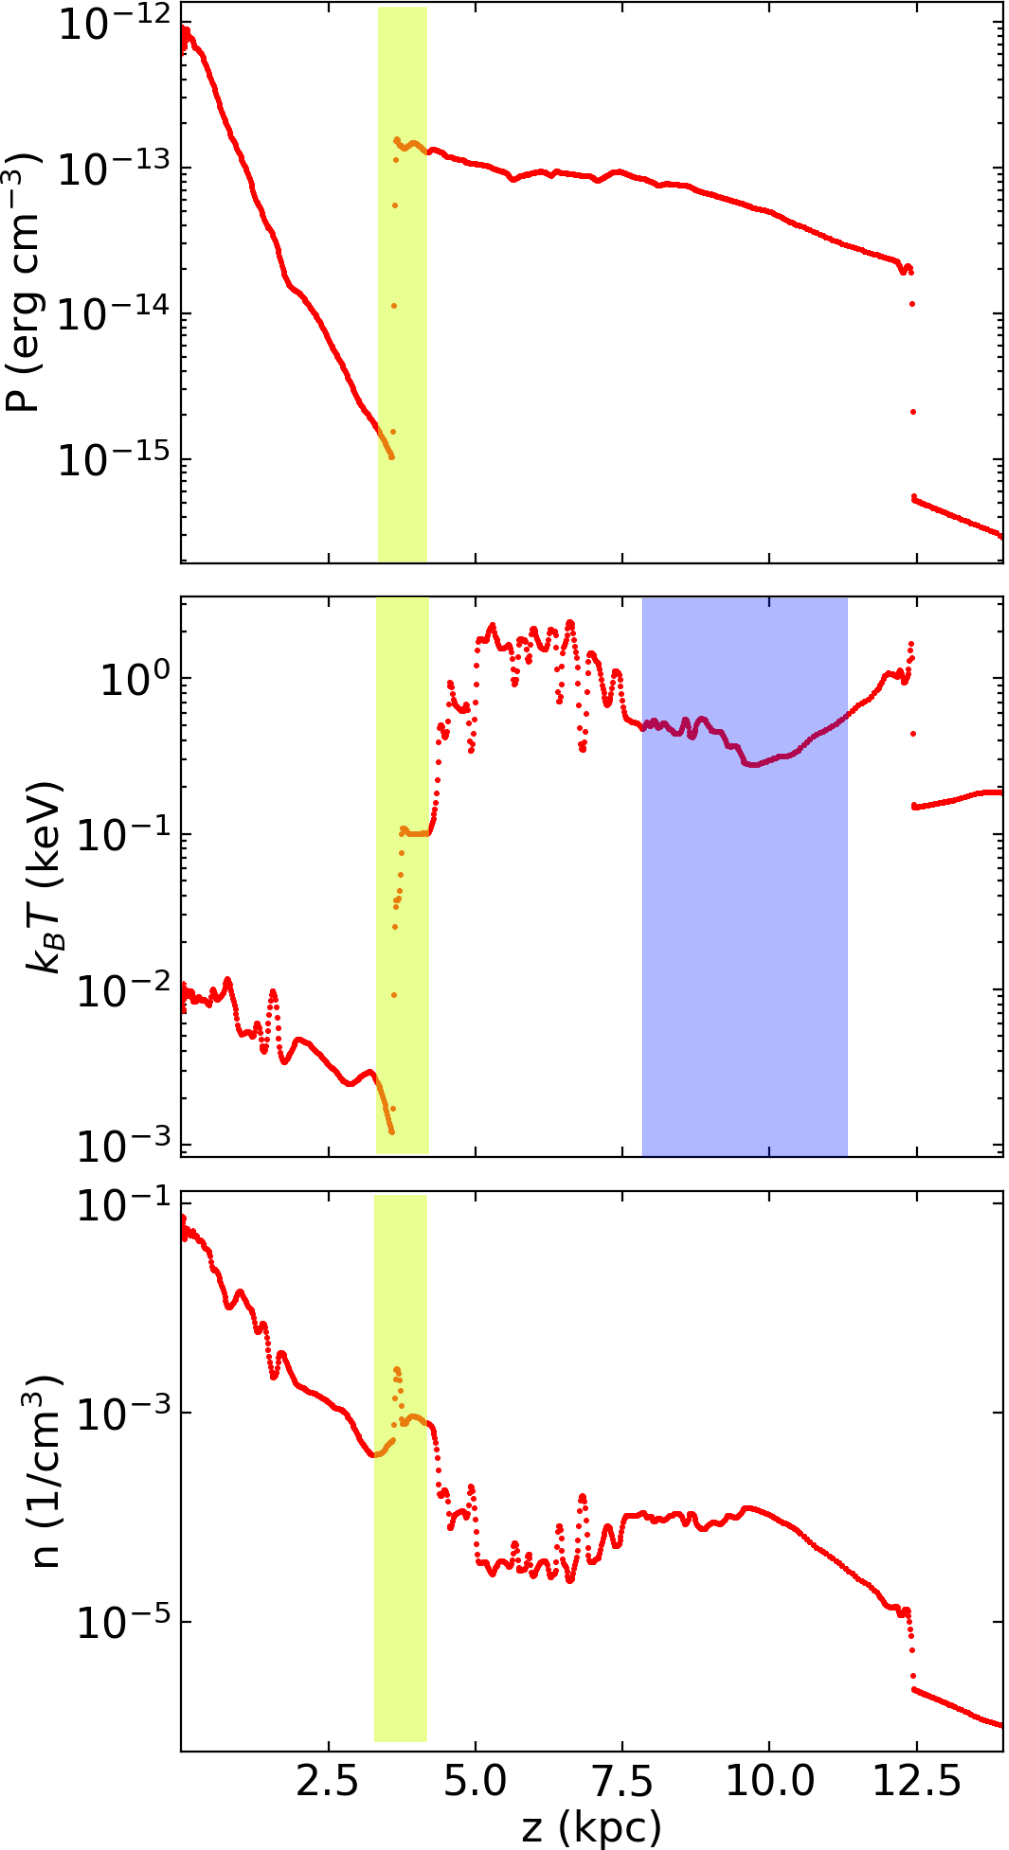
\includegraphics[height=8cm]{figures/fig__profile-1.png}%
         \label{fig__profile-1}%
      \end{subfigure}%
      \hspace{4pt}
      \begin{subfigure}[t]{0.5\linewidth}%
         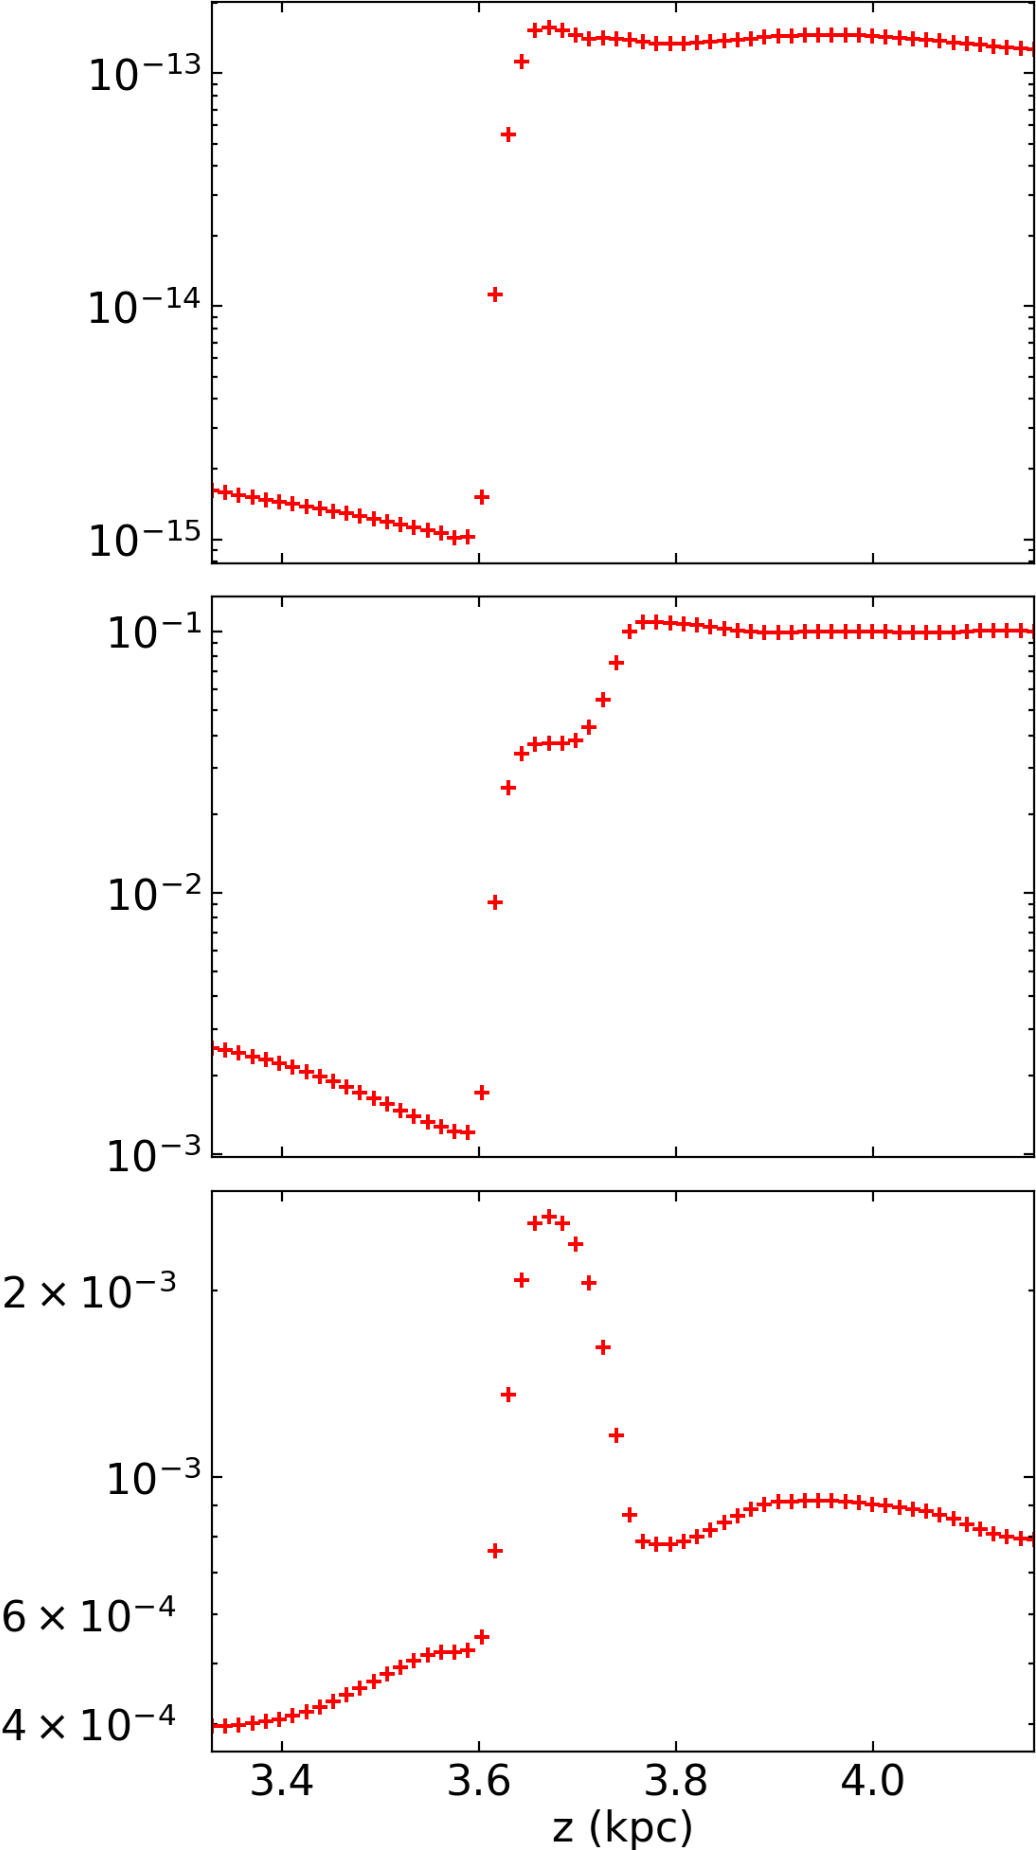
\includegraphics[height=8cm]{figures/fig__profile-2.png}%
         \label{fig__profile-2}%
      \end{subfigure}%
      \caption{
             Left: the profiles of pressure (top), temperature (middle),\
             and number density (bottom)\
             along the positive $z$-axis in Fig. \ref{fig__jetI5+ismSeed3-45deg}.
             Right: the close-up view of the profiles in the yellow band.\
             The sharp pressure jump at $z=3.62$ kpc\
             indicates that the innermost bubbles\
             (dashed box in the top panel in Fig. \ref{fig__jetI5+ismSeed3-45deg-a})\
             are an expanding reverse shock.
      }%
      \label{fig__profile}%
 \end{figure}%


  \begin{figure}
    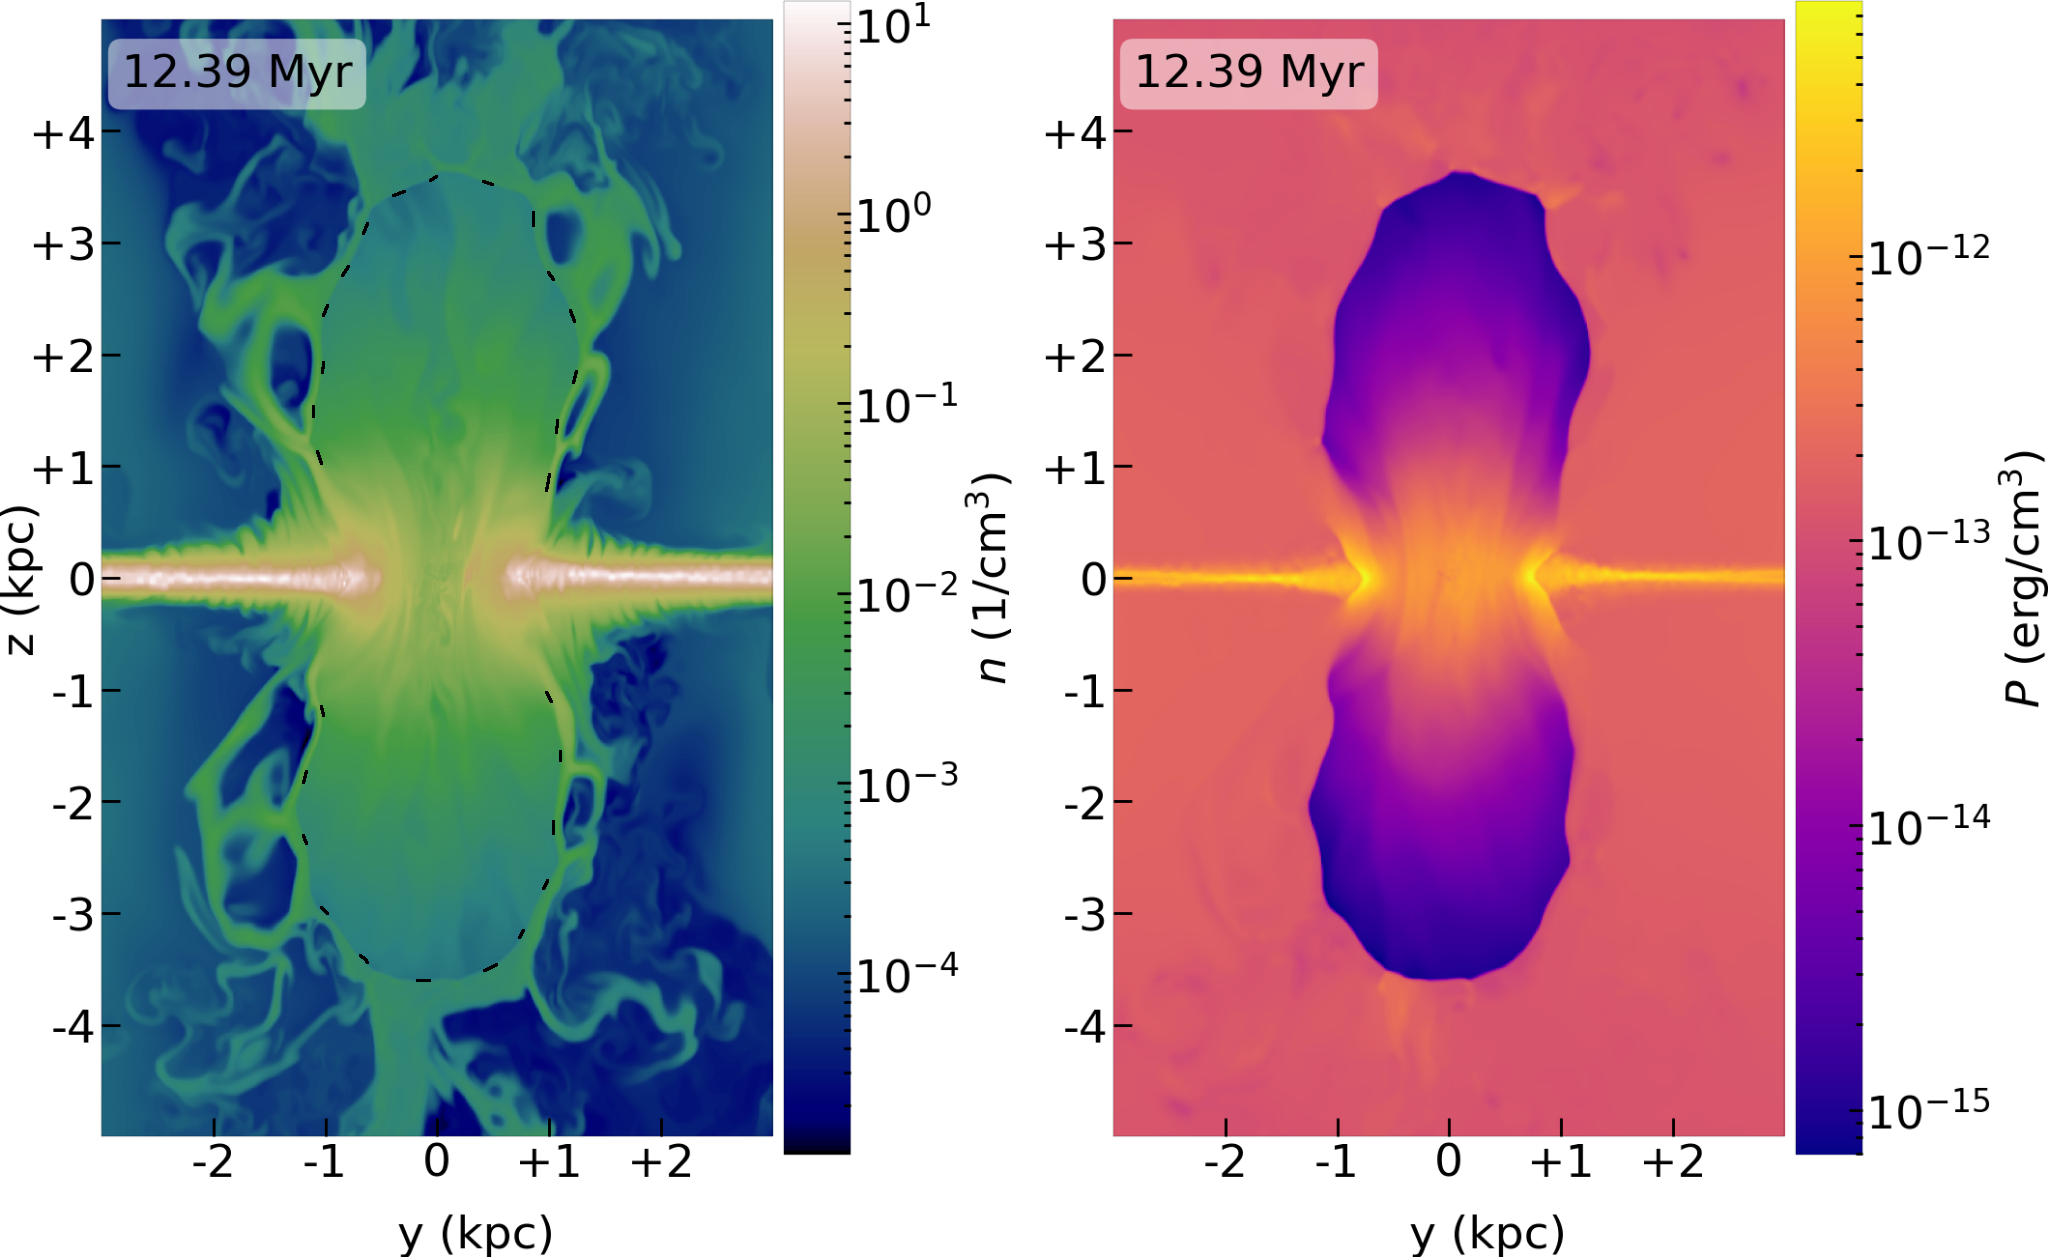
\includegraphics[width=\columnwidth]{figures/fig__innerbubbles.png}
    \caption{
       Zoom-in images of the density (left) and pressure (right) slices of the innermost bubbles.\
       The high density upstream of the reverse shock requires\
       an even higher density downstream.\
       Continuing outward, the higher density must match with low density further downstream;\
       thus there exists a dense shell\
       (the turbulent region outside the black dashed line on density slice).
     }
    \label{fig__innerbubbles}
  \end{figure}

  \subsection{Morphology and Profiles in X-ray}
  \label{X-ray}
  The X-ray emissivity is computed\
  for each computational cell
  using the MEKAL model \citep{Xray-1,Xray-2,Xray-3}\
  implemented in the utility XSPEC \citep{XSPEC}, assuming solar metallicity.\
  The X-ray intensity map is then generated by projecting the emissivities\
  along lines of sight\
  pointing away from the solar position at $(R_{\odot},0,0)=(8,0,0)$ kpc\
  with angular resolutions of 0.5 degrees, where $R_{\odot}$ is the Sun-GC distance.

  We point out that the projections used throughout this paper are \lq perspective\rq,\
  which has the effect of making a distant object appear smaller than the same object in a closer distance,\
  in order to facilitate a reliable interpretation of simulated all-sky map.\
  Also, the observed X-ray emission is contributed by all the gas in the Milky Way halo,\
  which likely extends to a radius of $\sim$250 kpc \citep{halo-radius-1,halo-radius-2},\
  much bigger than our simulation box. Therefore, we first compute the X-ray emissivity\
  from the simulated gas within a radius of 25 kpc away from the GC.
  Then, beyond 25 kpc the gas is assumed to be isothermal with $T=10^6$ K and\
  follows the observed density profile of \citep{temperature-MW} out to a radius of 250 kpc.

  Fig. \ref{fig__xray_0.8keV_angle_000} shows\
  the comparison between the simulated (top) and observed (bottom) all-sky map\
  in the range 0.6--1.0 keV.\
  In the simulated map, the red arrow at the center represents the direction of the bipolar jets,\
  constantly ejecting at an angle of $45^{\circ}$ to the disk normal between 0--1.2 Myr. Fig. \ref{fig__x-ray-profile-0.8keV-000} displays the simulated X-ray photon count rates as a function of Galactic longitudes (red)\
  in the same energy band as in Fig. \ref{fig__xray_0.8keV_angle_000}\
  cut at various Galactic latitudes (as labelled), compared with the observed profiles (black).

  {\color{red} KY: Please rewrite the following two paragraphs so that (1) the overall agreement between the simulated and observed bubble morphology and profiles are emphasized before discussing about discrepancies, and (2) some of the disagreement for the northern bubble could be due to the North Polar Spur. PH: done!}

  First, as shown in Fig. \ref{fig__jetI5+ismSeed3-45deg-a},\
  the half-width of the outermost bubbles is around 7 kpc,\
  corresponding to an half angular width $\sin^{-1}(7 \text{ kpc}/R_{\odot})\sim122^{\circ}$,\
  which is as wide as the eROSITA bubbles in the simulated X-ray map\
  (top panel in Fig. \ref{fig__xray_0.8keV_angle_000}).\
  We therefore suggest that the eROSITA bubble shells are a signature of compressed forward shocks\
  that have been driven into the northern and the southern Galactic halo,
  as previously proposed by \citet{Predehl2020} and \citet{Yang2022}. The broad agreement between simulated and observed X-ray maps hints that the full vertical extent of the eROSITA bubbles can be properly formed by an oblique jet within a thin disk of dense ISM.

  Second, we observe that\
  the simulated eROSITA bubbles are not as limb-brightened as the observation.\
  A possibility to enhance the X-ray emission is to include shock-accelerated CRs near the shock,\
  in which CRs could increase the compressibility of the fluid,\
  resulting in the enhanced thermal Bremsstrahlung emissivity that is proportional to density squared. Also, the disagreement for the northern bubble is expected as the North Polar Spur is generally thought to be caused by a remnant of a local supernova \citep{Egger1995}, which is not included in our simulations.


% 2. North Polar Spur is not shown as it is a supernova remanent near us.
  Third, the innermost bubbles\
  shown in Fig. \ref{fig__jetI5+ismSeed3-45deg},\
  even though with high column density, are invisible in the simulated X-ray map as\
  the temperature of the innermost bubbles is around $1$--$10$ eV\
  (see the temperature profile in Fig. \ref{fig__profile}).\
  Consequently, the X-ray emission within the innermost bubbles
  is severely suppressed by the cutoff $\exp\left[-h\nu/k_{B}T\right]$ in the thermal Bremsstrahlung emissivity.\
  This is the reason why the innermost bubbles are unseen in the X-ray observation.



 \begin{figure*}%
      \begin{subfigure}[t]{\textwidth}%
         \centering%
         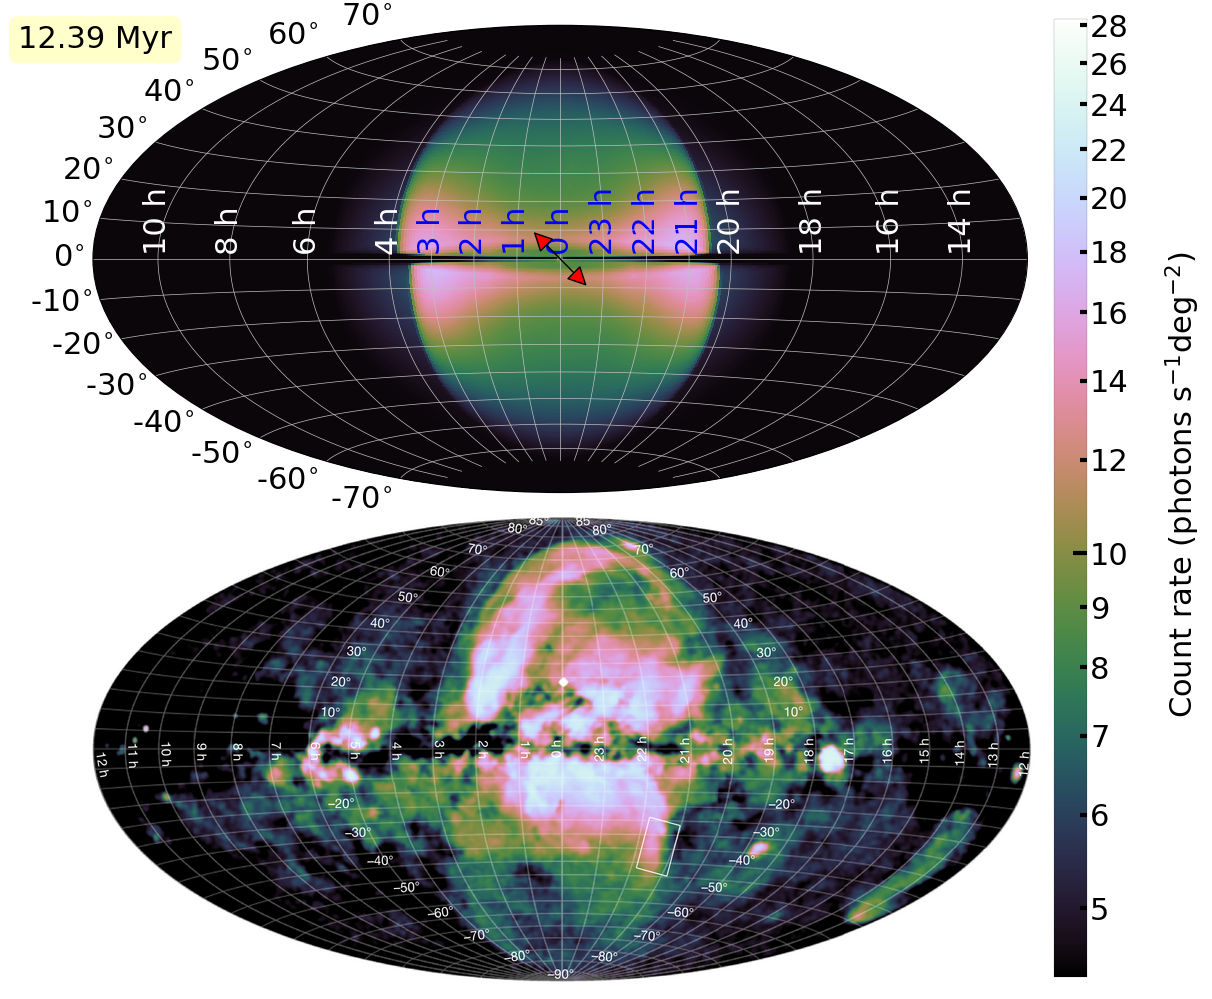
\includegraphics[width=0.85\textwidth]{figures/fig__xraymap.png}%
         \caption{
               Simulated (top) and observed (bottom; \citealt{Predehl2020}) count rate\
               (photons s$^{-1}$ deg$^{-2}$) in the 0.6--1.0 keV range.\
               Throughout this paper we show sky maps\
               in Galactic coordinates centered on the Galactic center using a Hammer-Aitoff projection.\
               %and observed from the solar system.\
               The red arrow at the center of the\
               top panel depicts the direction of the bipolar jets, constantly ejecting at an angle of $45^{\circ}$\
               to the disk normal for the first 1.2 Myr.
         }%
         \label{fig__xray_0.8keV_angle_000}%
         \end{subfigure}%
         \hspace{4pt}%
      \begin{subfigure}[t]{\textwidth}%
         \centering%
         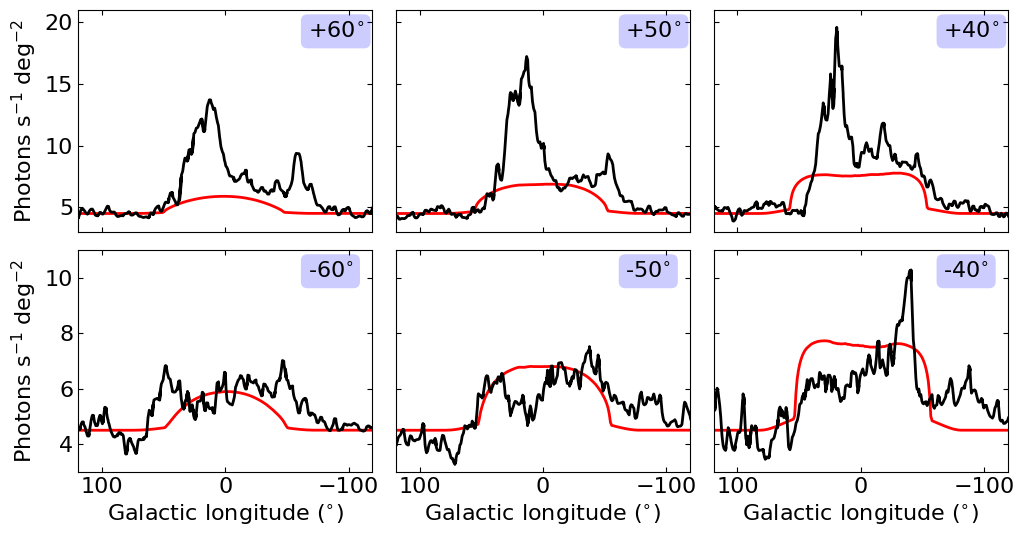
\includegraphics[width=0.85\textwidth]{figures/fig__xray-profile-0.8keV-000.png}%
         \caption{
               Comparison of the simulated (red) and observed (black; \citealt{Predehl2020}) one-dimensional photon\
               count-rate profiles in the same energy band as in Fig. \ref{fig__xray_0.8keV_angle_000},\
               cut at various Galactic latitudes (as labelled).
         }%
         \label{fig__x-ray-profile-0.8keV-000}%
      \end{subfigure}%
      \caption{}%
      \label{fig_xray-map}
 \end{figure*}%



\subsection{Gamma-ray and microwave spectra: constraint on the CRe spectral index}
\label{sec:gamma-ray-microwave}
In this section, we obtain the constraint on the CRe spectral index by\
comparing the simulated gamma-ray and microwave spectra\
with the observed spectra of the Fermi bubbles \citep{Ackermann2014}\
and the microwave haze \citep{Dobler_2008}, respectively.\

We assume the leptonic model for the gamma-ray and microwave emission as previous studies have shown that the bubble and haze spectra can be simulataneously produced by the same population of CRe \citep{Su2010, Ackermann2014, Yang2022}. In the leptonic scenario, the gamma-ray and microwave emission come from IC scattering of the ISRF and synchrotron radiation, respectively.\
Because the evolution of CR spectrum is not modelled in the simulations, we assume that the CRe spectrum is spatially uniform and follows a power-law distribution ranging from\
$0.5$ MeV ($\sim m_{\text{e}}c^2$) to $562.1$ GeV. The choice of $562.1$ GeV is motivated by\
the observed cutoff gamma-ray energy shown in Fig. \ref{fig__gammaRaySynchtronSpectrum}\
as most of the CRe energy is carried away by the up-scattered photons in the Klein-Nishina limit.


The IC emissivity of the upscattered photons at the energy $\epsilon_{1}$ is computed for\
each computational cell in our simulations\
using the Klein-Nishina IC cross-section \citep{Jones1968,BLUMENTHAL1970}\
to handle the scattering between ultra-relativistic CRe and photons in the ISRF:

\begin{subequations}
  \begin{align}
  &\frac{dE}{dtd\epsilon_{1}dV} =\nonumber\\
               &\frac{3}{4}\sigma_{T}c\mathbb{C}\epsilon_{1}\int^{\epsilon_{\text{max}}}_{\epsilon_{\text{min}}}
               \frac{n(\epsilon)}{\epsilon}d\epsilon\int^{\gamma_{\text{max}}}_{\gamma_{\text{min}}\left(\epsilon\right)}
               \gamma^{-(p+2)}f(q, \Gamma)d\gamma,\\
  \nonumber\\
  &f(q, \Gamma) =\nonumber\\
               &2q\ln q+(1+2q)(1-q)+0.5(1-q)\frac{\left(\Gamma q\right)^2}{1+\Gamma q},\\
  &q=\frac{\epsilon_{1}/\gamma\
               m_{\text{e}}c^{2}}{\Gamma\left(1-\epsilon_{1}/\gamma m_{\text{e}}c^{2}\right)},\\
  &\Gamma=\frac{4\epsilon \gamma}{m_{\text{e}}c^2},\\
  &\gamma_{\text{min}}(\epsilon)=\
   0.5\left(\frac{\epsilon_{1}}{m_{\text{e}}c^2}+\sqrt{\left(\frac{\epsilon_{1}}{m_{\text{e}}c^2}\right)^2+\
   \frac{\epsilon_{1}}{\epsilon}}\right) \label{gamma-min},
  \end{align}
\label{gammaray-emissivity}
\end{subequations}

where $\sigma_{T}$ is the Thomson cross section, $c$ is the speed of light,\
$m_{\text{e}}$ is the electron mass,\
$n(\epsilon)$ is the energy distribution of the photon number density in the ISRF given by \citet{Porter2017},\
$\gamma$ is the Lorentz factor of CRe, and\
$\mathbb{C}$ and $p$ are the normalization constant and spectral index of the CRe power-law spectrum.
$\gamma_{\text{min}}(\epsilon)$ is the minimum Lorentz factor of CRe\
that allows the incident photons to be scattered from energy $\epsilon$ to $\epsilon_{1}$, and\
$\gamma_{\text{max}}$ is the maximum CRe Lorentz factor in the spectrum. To obtain the simulated IC emissivities, we perform the double integration in Eq. \ref{gammaray-emissivity} on each cell\
over the range of the CRe Lorentz factor and\
the range of incident photon energy between\
$\epsilon_{\text{min}}=1.13\times10^{-4}$ eV (cosmic microwave background) and\
$\epsilon_{\text{max}}=13.59$ eV (optical starlight).\


The synchrotron emissivity with an isotropic electron pitch angle distribution\
is given by \citet{BLUMENTHAL1970}:

\begin{subequations}
   \begin{align}
      &\frac{dE}{dtd\nu dV} =\nonumber\\
      &\frac{4\pi\mathbb{C}e^{3}B^{0.5(p+1)}}{m_{\text{e}}c^{2}}\
      \left(\frac{3e}{4\pi m_{\text{e}}c}\right)^{0.5(p-1)}\
      a(p)\nu^{-0.5(p-1)},\\
      &a(p)=\nonumber\\
           &\frac{2^{0.5(p-1)}\sqrt{3}\Gamma\left[\left(3p-1\right)/12\right]\
                                      \Gamma\left[\left(3p+9\right)/12\right]\
                                      \Gamma\left[\left(p+5\right)/4\right]}
      {8\sqrt{\pi}(p+1)\Gamma\left[\left(p+7\right)/4\right]},
   \end{align}
   \label{synchrotron-emissivity}
\end{subequations}

where $\Gamma$ is the gamma function, and $B$ is the magnetic field strength defined in\
Eq. \ref{magnetic-field}. For a given longitude and latitude range, the simulated spectra are\
computed by projecting emissivities\
as we project X-ray emissivities in Section \ref{X-ray},\
and then we average the spectra over all the sight lines within the region on the sky.


Fig. \ref{fig__gammaRaySynchtronSpectrum} shows the simulated microwave (left)\
and gamma-ray (right) spectra averaged over the different patches (shown in the legends) of the sky.\
The rows from top to bottom show the spectra with different assumptions of the CRe spectral index, $2.2, 2.4$ and $2.6$.\
We highlight our findings as follows.\

First, we find that, among the three values of the CR spectral indices assumed, a CRe spectral index of 2.4 (the middle row) provides the best fits for both the the simulated gamma-ray spectra as well as the microwave spectra. This value is slightly steeper than the best-fit spectral index of $\sim 2.17$ found by \cite{Ackermann2014}. However, we note that our calculation takes into account the 3D variations of the ISRF, whereas the previous constraint was based on the ISRF at a fixed height of 5 kpc away from the Galactic plane.

Second, the simulated gamma-ray spectra are\
nearly latitude independent. Note that we have assumed spatially uniform spectrum for the underlying CRe, and hence the simulated gamma-ray spectra at different latitudes mainly reflect how the 3D distribution of the simulated CR number density (see Fig. \ref{fig__jetI5+ismSeed3-45deg-CR})  is projected into different latitude bins. Overall we find good agreement between the simulated and observed spectra \citep{Ackermann2014}; only the simulated spectrum at high latitudes tends to be slightly dimmer than the lower-latitude spectrum because the optical intensity in the ISRF decays with increasing latitudes.

Third, our assumed range for the CRe spectrum (0.5 MeV to 562.1 GeV) produces gamma-ray spectra with a high-energy cutoff around energies 400--500 GeV,\
consistent with the observed cutoff energy.\
This is expected since\
the upscattered high-energy photons ($\epsilon_{1}\sim450$ GeV) mainly arise from\
the scattering between the relativistic CRe ($\gtrapprox 408$ GeV)\
and optical starlight ($\epsilon \sim 10$ eV).\
Thus, Eq. \ref{gamma-min} can be reduced to $\epsilon_{1}\sim\gamma m_{\text{e}}c^2$\
in the Klein--Nishina limit\
$\left(\text{i.e. }\epsilon_{1}\epsilon \gg \left(m_{\text{e}}c^2\right)^2\right)$,\
implying most of the CRe energy is carried away by the upscattered photons.

Finally, the good agreement between the simulated and observed gamma-ray/microwave spectra\
implies that, in the presence of ISRF and magnetic fields, the emission of the Fermi bubbles and\
the microwave haze can be produced by the same high-energy electrons\
via IC scattering and synchrotron radiation, respectively. Our results thus provide further support for the leptonic model as previously suggested \citep{Su2010, Ackermann2014, Yang2013, Yang2022}.

\begin{figure*}
  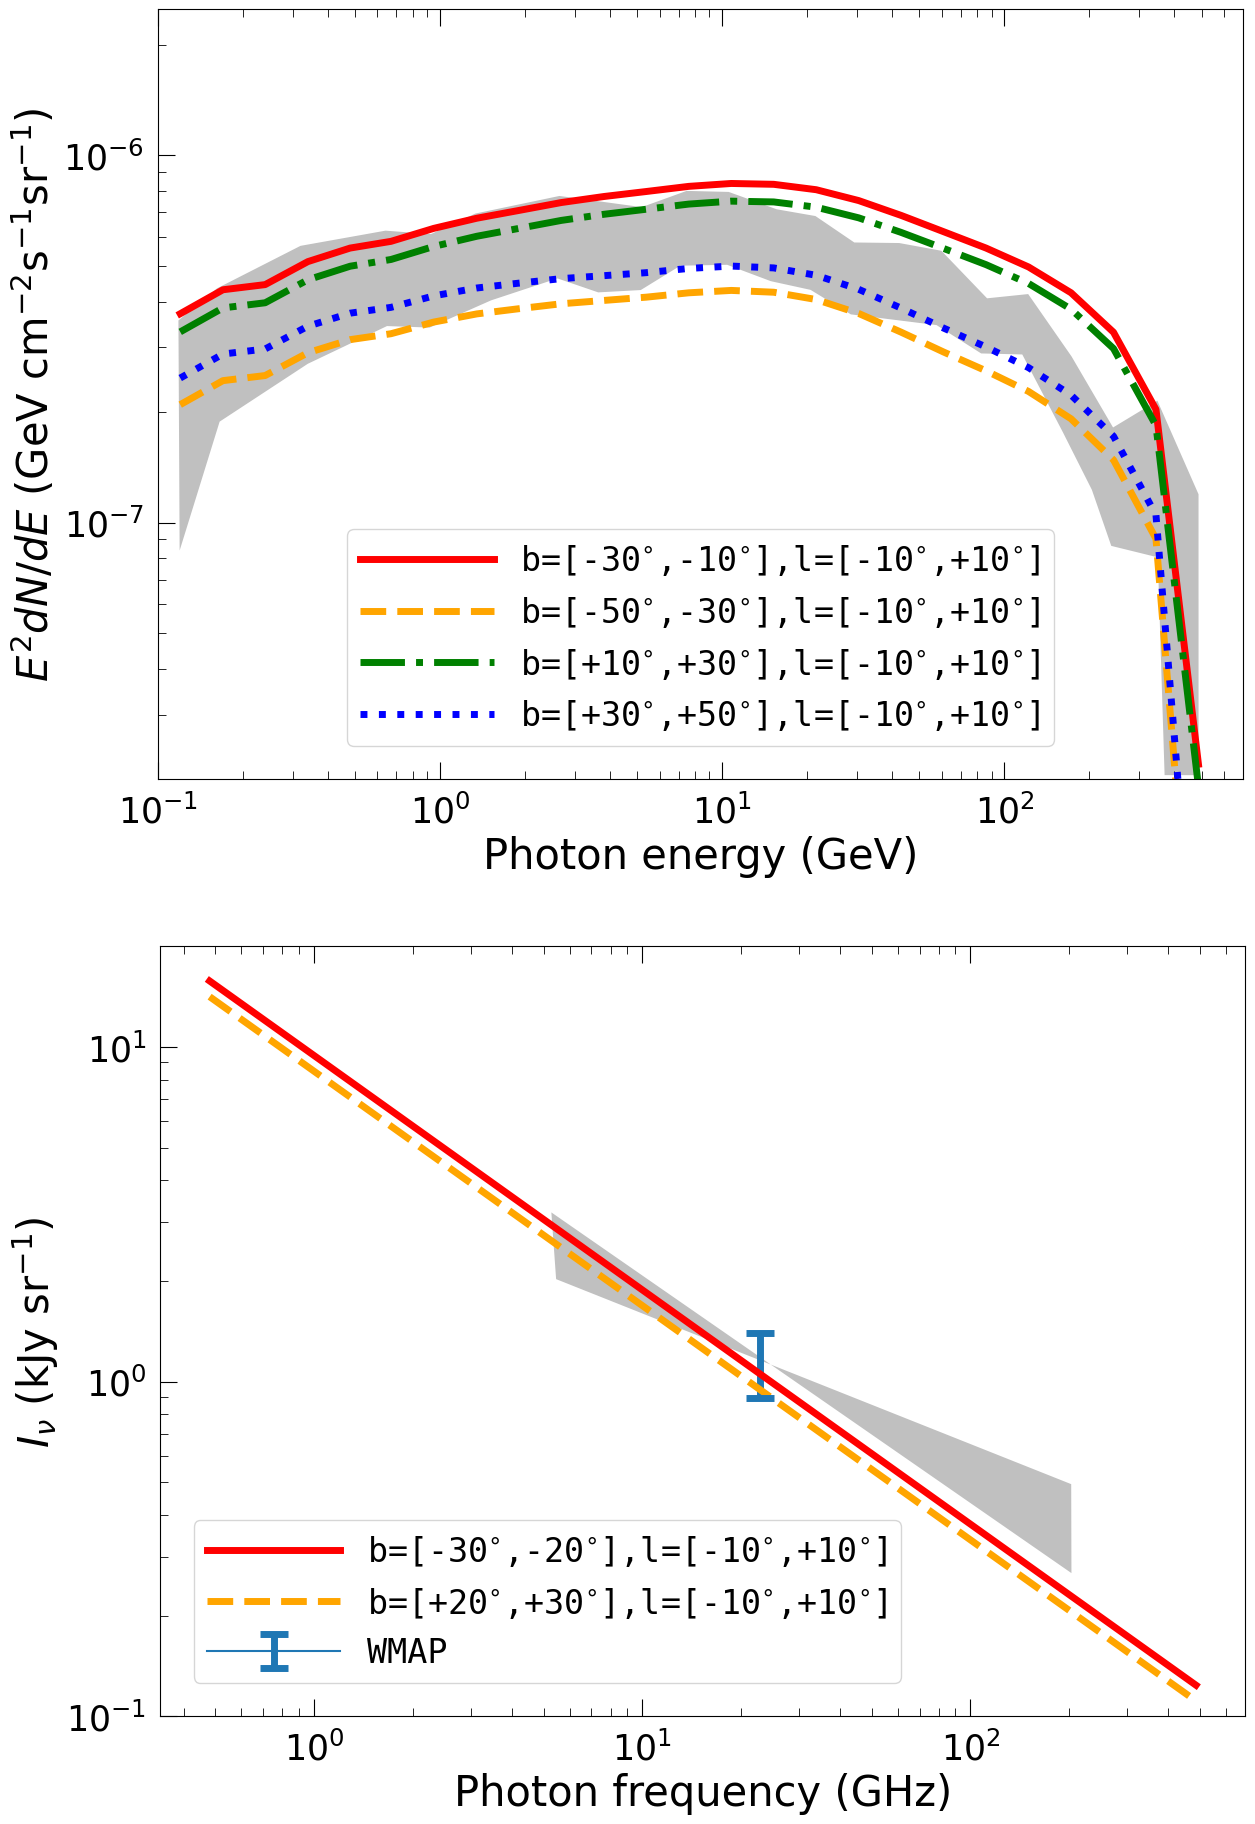
\includegraphics[width=\linewidth]{figures/fig__spectrum.png}
  \caption{
      Simulated microwave spectra (colored lines in left) averaged over $20^{\circ}<|b|<30^{\circ}$, $|l|<10^{\circ}$.\
      The data point represents the \textit{WMAP} data in the 23 GHz K band and\
      the shaded bow-tie area indicates the range\
      of synchrotron spectral indices allowed for the \textit{WMAP} haze \citep{Dobler_2008}.\
      Simulated gamma-ray spectra (colored lines in right column)\
      of the \textit{Fermi} bubbles calculated for a longitude range of\
      $|l|<10^{\circ}$ for different latitude bins.\
      The gray band represents the observational data of \citet{Ackermann2014}.\
      The row from top to bottom shows the microwave (left) and gamma-ray (right) spectra\
      with CRe spectral index $2.2, 2.4$ and $2.6$, respectively.\
      The CRe cutoff energy is 562.1 GeV in all cases.
  }
  \label{fig__gammaRaySynchtronSpectrum}
\end{figure*}

 Fig. \ref{fig__gammaRay-map} shows the simulated gamma-ray photon flux with a CRe power-law index 2.4\
 compared with the observed one\
 in the energy bin $76.8-153.6$ GeV.\
 As the eROSITA bubbles,\
 one can see that the symmetric \textit{Fermi} bubbles\
 can also be realized by oblique jets. The extent of the simulated gamma-ray bubbles is also comparable to the observed ones.\
 However, we find that the simulated bubble surface is not as smooth
 as the observed bubbles. The instabilities at the bubble
 surface may be suppressed by the magnetic draping
 effect \citep{Lyutikov2006,Yang2012} if magnetic fields were
 included in the simulations. With magnetic draping, the sharp edges of the observed bubbles \citep{Su2010, Ackermann2014} could also be explained by anisotropic CR diffusion along field lines \citep{Yang2013}.

 The simulated gamma-ray intensity
 distribution is shown in Fig. \ref{fig__gammaRay-map}. Though the overall size of the simulated gamma-ray bubbles is comparable to that of the observed ones, the gamma-ray intensity does not appear to be
 as uniform as originally found in \citet{Su2012}.
 As discussed above, the gamma-ray intensity is slightly
 higher close to the Galactic plane due to the stronger
 radiation field at lower latitudes. However, this level
 of brightness variations appears to be consistent with the later
 observational data of \citet{Ackermann2014} and \citet{Selig2015}, which shows that there are some substructures in the gamma-ray intensity distribution within the bubbles.

 For completeness, we show the simulated CR energy density at 12.39 Myr in Fig. \ref{fig__jetI5+ismSeed3-45deg-CR}. The comparison between\
 Fig. \ref{fig__jetI5+ismSeed3-45deg}\
 and\
 Fig. \ref{fig__jetI5+ismSeed3-45deg-CR}\
 shows that the CR pressure\
 is around 5$\times10^{-15}$--8$\times10^{-15}$ erg cm$^{-3}$,\
 bringing the CR-to-gas pressure ratio is 0.1--0.2,
 similar to 0.18 at the beginning of the simulation.
 We therefore stress that\
 ignoring the contribution of CR pressure gradient to the momentum of the gas\
 in Eq. \ref{governing-eq} is reasonable.




\begin{figure*}
  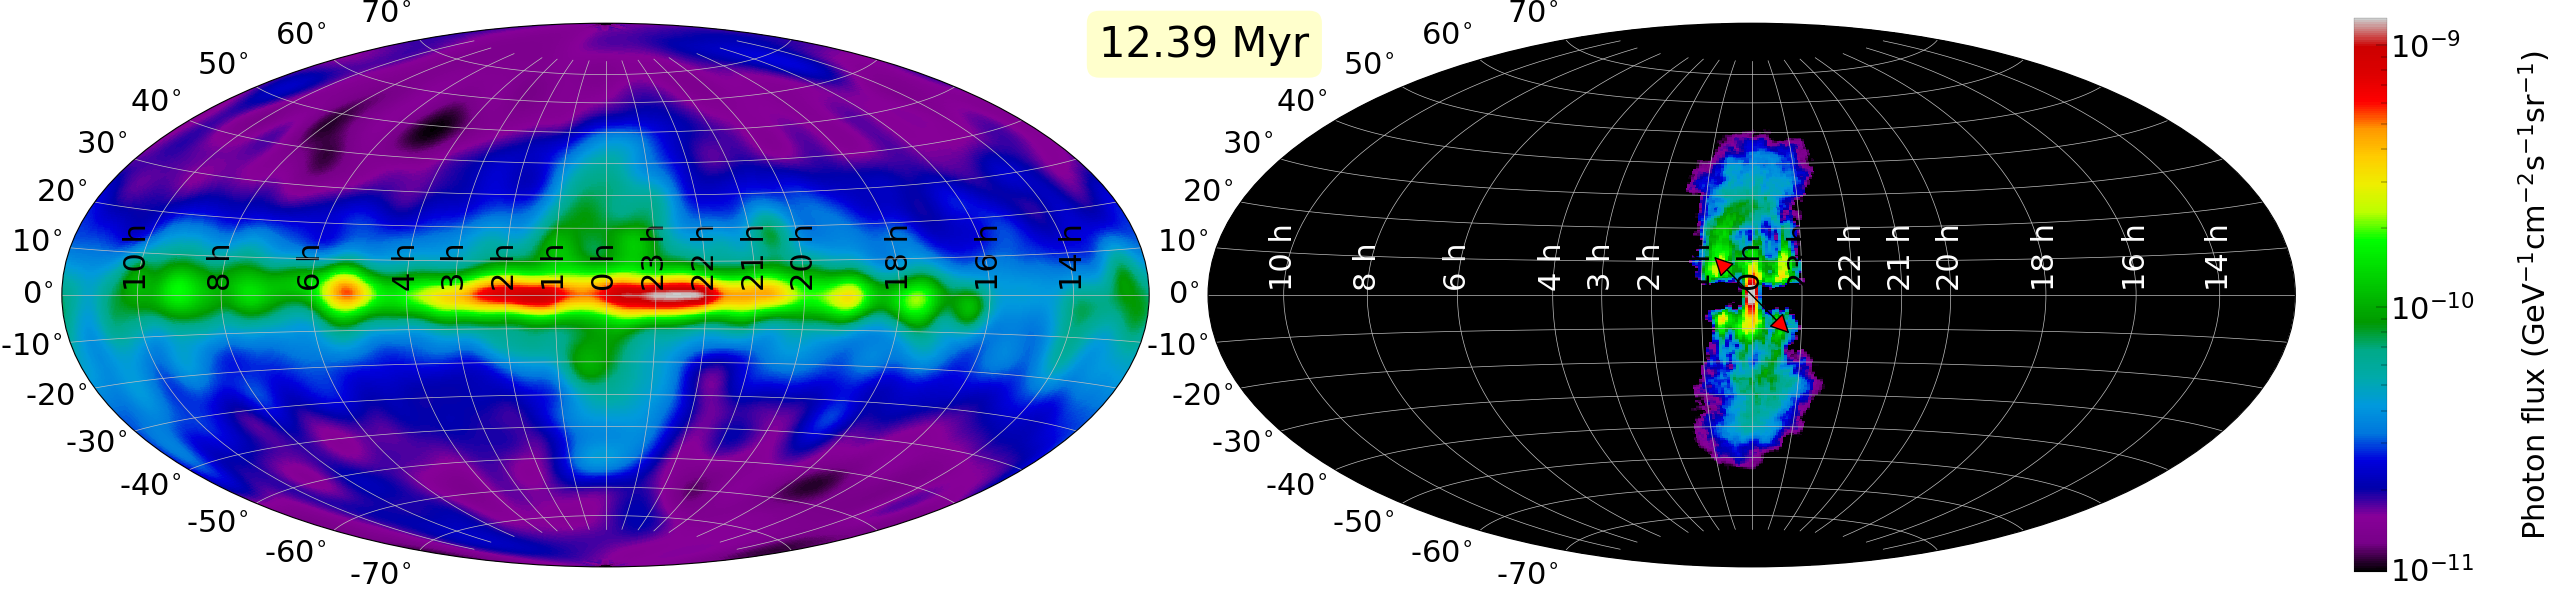
\includegraphics[width=\linewidth]{figures/fig__GammaRay_100e9_1e6_angle_000.png}
  \caption{The observed (left; \citealt{Selig2015}) and simulated (right) photon flux\
           in the energy bin $76.8-153.6$ GeV.\
           Note that the left panel is the\
           photon flux of the diffuse component reconstructed by the D$^3$PO\
           algorithm \citep{Selig2015} that analyzes\
           the photon data from the \textit{Fermi} Large Area Telescope \citep{Atwood2009}\
           and removes the contribution from point-like component.
           The red arrow at the center of the right\
           panel depicts the direction of the bipolar jet, constantly ejecting at an angle of $45^{\circ}$\
           to the disk normal in 1.2 Myr.
  }
  \label{fig__gammaRay-map}
\end{figure*}



  \begin{figure}
    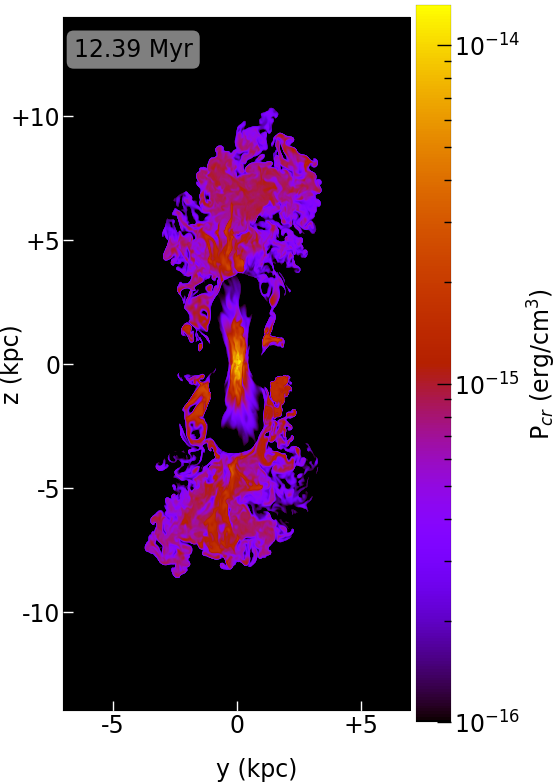
\includegraphics[width=\columnwidth]{figures/fig__jetI5+ismSeed3-45deg-CR.png}
    \caption{
     The CR pressure slice passing through the jet source at 12.39 Myr.\
     Comparison between\
     gas pressure (Fig. \ref{fig__jetI5+ismSeed3-45deg}) and cosmic ray pressure\
     shows that
     the CR pressure\
     is around 5$\times10^{-15}$--8$\times10^{-15}$ erg/cm$^{3}$,\
     bringing the CR-to-gas pressure ratio is 0.1--0.2,
     similar to 0.18 at the beginning of the simulation.
     We therefore stress that\
     ignoring the contribution of CR pressure gradient to the momentum of the gas\
     in Eq. \ref{governing-eq} is reasonable.
     }
    \label{fig__jetI5+ismSeed3-45deg-CR}
  \end{figure}

\section{Discussion}
Our modeled gamma-ray and microwave spectra assumed that
the underlying CRe spectrum is spatially uniform.
Therefore our results imply that, whatever the true re-acceleration and cooling mechanisms are,
the CRe spectrum at the present time has to be spatially uniform with
a spectral index of 2.4 in order to fit the observed spectra.







\section{Conclusions}
\label{Conclusions}
In this work, we introduce a thin, dense disk composed of clumpy ISM\
to divert the oblique jets at an angle $45^{\circ}$\
to the disk normal in the past energetic event of the central SMBH in the Milky Way Galaxy.\
We investigate the properties of the Galactic bubbles and the microwave\
haze using 3D SRHD simulations of CR jet injections from\
the SMBH assuming the leptonic model. The important findings are summarized as follows.

\begin{itemize}

\item The Galactic bubbles are nearly symmetric about the Galactic plane albeit\
      the bipolar jets are at an angle $45^{\circ}$\
      with respect to the disk normal.\
      We showed that inclusion of the dense ISM disk (regardless of its clumpiness) is a critical component for producing the symmetric Galactic bubbles when the jets are oblique.\
      The broad agreement between the simulated and observed multi-wavelength features\
      demonstrates that oblique jets are a plausible scenario of forming the Galactic bubbles, which\
      releases the caveat of earlier jet models that the jets must be vertical to the Galactic plane.\


%\item The randomness of the clumpy disk has an insignificant impact on the overall dynamic of the Galactic bubbles.\
%      The development of the reverse shocks (the innermost bubbles) is always associated with the dense disk,\
%      without the disc, the outermost bubbles and the turbulent plasma will be oblique,\
%      indicating the dense disc is crucial for\
%      the symmetry of the Galactic bubbles and for the innermost bubbles formation.
      {\color{red} KY: I removed the second point about the innermost bubbles for now, because I think the following two points should be separated: (1) inclusion of the disk is critical for forming symmetric Galactic bubbles, (2) we found a pair of innermost bubbles which are reverse shocks (and perhaps comment on their properties and/or observable signatures).}
\item The development of the expanding forward-reverse shock pair is always associated with the dense disk. Also, without the thin disk, only forward shocks exist. The forward-reverse shock pair heats the turbulent plasma up considerably ($\sim2$ keV) as the plasma is bracketed between their downstream. There exists a dense shell that fits closely to the reverse shock because the gas is immediately compressed as it passes outward through the reverse shock while coinciding with the low gas density further downstream.

\item In the oblique jet scenario, the edge of the eROSITA bubbles is a forward shock,\
      originally driven by oblique bipolar jets emanating from the GC 12.39 Myr ago for a duration of 1.2 Myr\
      and significantly expanded within the stratified atmosphere afterwards.\
      The overall extent of the simulated X-ray bubbles is comparable to that of the eROSITA bubbles, though not as limb-brightened.\
      Future models including shock-accelerated CRs may help to resolve this issue by increasing the compressibility of the fluid and enhancing the thermal Bremsstrahlung emissivity at the edge of the X-ray bubbles.
      %The simulated eROSITA bubbles are not as limb-brightened as the observation.\
      %A possibility to enhance the X-ray emission is to include shock-accelerated CRs near the shock,\
      %in which CRs could increase the compressibility of the fluid,\
      %resulting in the enhanced thermal Bremsstrahlung emissivity that is proportional to density squared.
\item Followed by the forward shock is a turbulent, hot plasma ($\sim2$ keV) filled with the injected CRs in pressure balance with the shocked medium, which we interpret as the \textit{Fermi} bubbles.\
      The similarity of the morphology, temperature, and gamma-ray spectrum between\
      simulated and observed bubbles suggests that\
      the edge of the \textit{Fermi} bubbles are likely associated with the contact discontinuity between the turbulent, hot plasma and the post-shock medium. The surface of the simulated bubbles is not as smooth as the observed ones; inclusion of magnetic fields in the future may help suppress the instabilities at the bubble surface due to the mangetic draping effect.
\item Assuming a leptonic model with a spatially uniform, power-law CRe spectrum ranging from 0.5 MeV to 562.1 GeV, we showed that the observed gamma-ray and microwave spectra can simultaneously reproduced. The best-fit\
      CRe power-law index is found to be 2.4.
\item Associated with the Galactic magnetic field\
      will lead to the stochastic acceleration of CRe, possibly in balance with the IC and synchrotron cooling.\
      We will investigate the competition between stochastic acceleration and radiative cooling in a future work. {\color{red} KY: This item is to be modified according to the newly added text in the Discussion section.}
\end{itemize}



\section{Acknowledgements}
The authors thank Mateusz Ruszkowski and Ellen G. Zweibel for insightful comments.\
We thank Peter Predehl for providing the range of observed X-ray intensity in Fig. \ref{fig__xray_0.8keV_angle_000}.\
A part of the simulations are performed and analyzed using computing resources\
operated by the National Center for High-Performance Computing (NCHC).
HYKY acknowledges support from\
Yushan Scholar Program of the Ministry of Education of Taiwan\
and\
Ministry of Science and Technology of Taiwan (MOST 109-2112-M-007-037-MY3).
HS acknowledges\
funding support from the Jade Mountain Young Scholar Award No. NTU-109V0201,\
sponsored by the Ministry of Education, Taiwan.\
This research is partially supported by the Ministry of Science and\
Technology of Taiwan (MOST) under grants MOST 107-2119-M-002-036-MY3\
and MOST 108-2112-M-002-023-MY3, and the NTU\
Core Consortium project under grants NTU-CC-108L893401 and\
NTU-CC-108L893402.

\section*{Data Availability}
The data underlying this article are available in the article and in its online supplementary material.

%%%%%%%%%%%%%%%%%%%% REFERENCES %%%%%%%%%%%%%%%%%%

% The best way to enter references is to use BibTeX:

\bibliographystyle{mnras}
\bibliography{paper} % if your bibtex file is called example.bib


\appendix
\section{jets parameter variations}
\textcolor{red}{KY: Please also add a section (either in the Discussion
or Appendix) to discuss about the parameter variations.
I think the figures you showed me are very important
and informative.}



%%%%%%%%%%%%%%%%% APPENDICES %%%%%%%%%%%%%%%%%%%%%
\end{document}

% End of mnras_guide.tex

